%IMPORTANT!!!!!! remember to abilitate twoside, openright to print document.
%remember the clearpages for editing better.

\documentclass[12pt]{report}%, twoside, openright]{report}
\usepackage[english]{babel}
\usepackage[utf8]{inputenc}
\usepackage{amsmath}
\usepackage{graphicx}
\graphicspath{{diagrams/}}
\usepackage{listings}
\usepackage{dirtytalk}

\usepackage[backend=biber,
						bibstyle=ieee,
						sorting = nty,
						citestyle=numeric-verb]{biblatex}
\bibliography{bibliography.bib}
\begin{document}

\begin{titlepage}

\newcommand{\HRule}{\rule{\linewidth}{0.5mm}}


\includegraphics[width=6cm, height=2cm]{fhlogo}
\vfill
\center % Center everything on the page
\textsc{\LARGE Fachhochschule Dortmund}\\[1.5cm] % Name of your university/college
\textsc{\Large Master's Thesis}\\[0.5cm] % Major heading such as course name

\HRule \\[0.4cm]
{\large \bfseries Development of a real-time software architecture for AMiRo robot based on the operator controller-module}\\[0.4cm]
\HRule \\[1.5cm]

\begin{minipage}{0.4\textwidth}
\begin{flushleft} \large
\emph{Author:}\\
Hector Gerardo Munoz Hernandez
\end{flushleft}
\end{minipage}
~
\begin{minipage}{0.4\textwidth}
\begin{flushright} \large
\emph{Supervisors:} \\
Prof. Dr. Carsten Wolff

Uwe Jahn
\end{flushright}
\end{minipage}\\[2cm]

\large \textit{A thesis submitted in fulfilment of the requirements\\ for the degree of Master of Engineering (M.Eng.)\\ in Embedded Systems for Mechatronics}\\[0.3cm]

{\large \today}\\[1cm]

\vfill
\end{titlepage}

\pagenumbering{roman}
\tableofcontents
\listoffigures
\listoftables

\begin{abstract}
The objective of this project is to develop and implement a software architecture that fulfills the real-time system requirements. The development and implementation are done for the Autonomous Mini Robot or AMiRo. This thesis starts discussing the hardware structure of the robot, and the review and analysis of the AMiRo OS that was done in the University of Bielfield. The AMiRo OS was replaced by a software solution that uses the \textit{Operator Controller Module} approach. This software solution is called the DA\_AMiRo project and it discussed over the next few chapters as it is the main part of the thesis. The purpose of this software architecture is to build a real-time scheduler for the values of the sensors and actuators that AMiRo has and are communicated via the Controller Area Network protocol. There are also some sample applications and demos that show the functionality of the DA\_AMiRo. The thesis ends with a comparison between the AMiRo OS and the DA\_AMiRo project. The entire DA\_AMiRo project can be found in the gitlab repository \cite{AMiRo_Git}. As for the AMiRo OS project, the reader can also get access to the complete codes in the AMiRo Wiki \cite{AMiRo_Wiki}.

\end{abstract}
\pagenumbering{arabic}

\chapter{Introduction}
\section{Real-time Operating Systems}
The necessity to meet deadlines in today's projects is growing constantly. Most applications consist of different tasks that can be executed in parallel, have different priority, have different repetition period, and frequently use shared resources. Using a multi-threading approach, however, can create a challenge in terms of performance, stability and time of implementation.

An operating system is a software component of a computer system that is responsible for the management and coordination of activities and the sharing of the resources of the computer \cite{mcgraw}. "A real-time operating system perform these tasks, but is designed to run applications with a very precise timing and a high degree of reliability. This can be especially important in measurement and automation systems where downtime is costly or a program delay could cause a safety hazard" \cite{rtos}.

In other words, a real-time operating system is an operational system that provides certain capability according to preset timing constraints \cite{whatisRTOS}. This is achieved through a scheduler that is designed to provide a deterministic execution pattern. And so, the RTOS are used in systems with critical timing requirements, when each task should be executed within a restricted time interval \cite{whatisRTOS}.

When it can be guaranteed that a task will never exceed a maximum amount of time in being completed, it can be said that the operative system is "hard real-time". If it can be guaranteed that a task will most of the time not exceed a maximum amount of time in being completed, it can be said that the operative system is "soft real-time". An airbag system is an example of a "hard real-time" system, where the task has to be guaranteed to execute always within a time limit. For a "soft real-time" example, a video streaming can be considered, where an occasional loss of data can be accepted because it does not compromise the whole functionality \cite{rtos}.

In the real-time operating systems the managing of the tasks is crucial. To this end, programmers have to decide which task is running at certain time and how other tasks can preempt the processing resources if their priorities are higher. In other words, manage the schedule of the tasks so that they meet with their deadlines.

Some of the main characteristics of a RTOS are the following:

\begin{itemize}
\item Determinism: An application timing can be guaranteed within a certain margin of error.
\item Soft and Hard Real-Time: The validity of data after meeting a deadline. In soft real-time the deadline is not that crucial but in hard real-time the meeting of the deadline is very important.
\item Jitter: Which is the amount of error in the timing of a task over subsequent iterations of a program or loop \cite{whatisRTOS}.
\end{itemize}

\section{Operator Controller Module}

The DA\_AMiRo software architecture is based on the OCM \cite{ocmAuto} software architecture approach. In this structure there are three basic controllers: Internal Controller, Reflective Operator, and Cognitive Operator. In order to have a more precise overview of how these three controllers work, figure \ref{fig:ocm} is explained by a direct quote from the Wiki:

\say{Refering to figure \ref{fig:ocm}, the Controllers (red) are used to connect all sensors and actuators. The Controllers need to be configured and programmed once, so the software on the controllers is mostly fixed and does not need to be flexible. The Reflective Operator(s) (yellow) control the Controllers. The Reflective Operator's software is the adaptable part of the distributed system - it changes from application to application. These Operator Controller Module(s) are located on the robot itself and let it act autonomously. The Cognitive Operator is hosted on a server and is used to optimize, program and interact with the user. The Cognitive Operator is connected via a wireless connection and can (only) interact with the Reflective Operator(s).}\cite{DAEbot_Wiki}.

\begin{figure}[h!t]
	\centering
	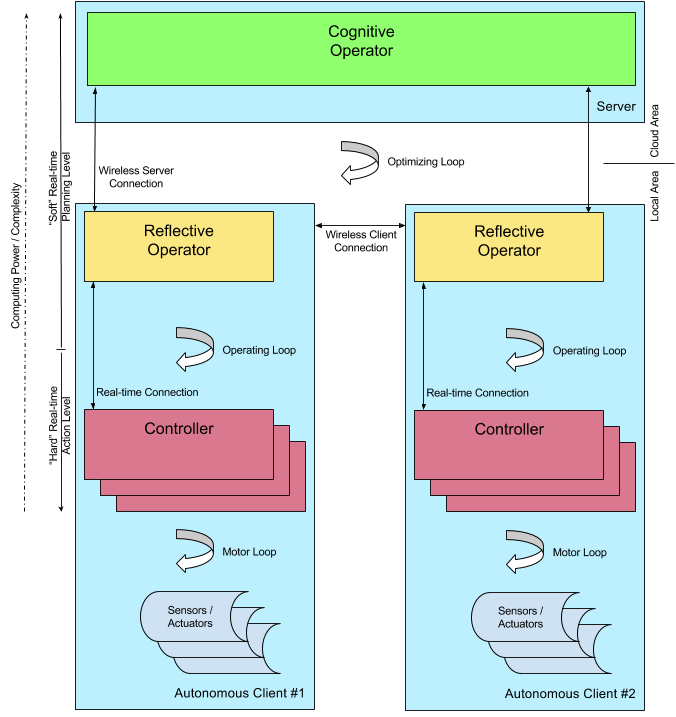
\includegraphics[width=\textwidth]{ocm}
    \caption{OCM software arquitecture for the DAEbot\cite{DAEbot_Wiki}.}
    \label{fig:ocm}
\end{figure}
\clearpage

The OCM was introduced by a group of Professors in the University of Paderborn. The concept aimed to structure and design a reconfigurable controller systems \cite{ocmAuto}. As mentioned before, there are three different levels in the OCM. The first one is the lowest level of the OCM also simply known as the Controller. This level interacts directly with the plant of the system, which means that the control signal is produced and measured here. It is also necessary that the software processing in this layer is quasi-continuous so that the measured values are processed in real-time conditions \cite{ocmAuto}.

The second layer is called the reflective operator. It is in this layer where the monitoring and the controlling routines are executed \cite{ocmAuto}. This layer does not have access to the actuators directly, because the Controller is already doing this. The expected result is that the Reflective Operator modifies the Controller, sometimes also changing between different pre-established Controller configurations. This level also requires a quasi-continuous operations like a continuous adaptation algorithm or a watchdog. This operator also has to operate under hard-time constraints because its relation with the Controller. In short, this layer serves as a interface between the Cognitive Operator and the Controller \cite{ocmAuto}.

The third layer is the Cognitive Operator. On this layer the system gathers information about itself and its environment to improve itself. This recollection of information can be done by applying various methods such as learning and model-based optimization among others. In other words, it is in this layer where the self-improvement takes place \cite{ocmAuto}.

This project compares the AMiRo OS with the OCM based architecture of the DA\_AMiRo. The controller is the responsible for commanding the internal sensors of the STM32F32 boards inside DA\_AMiRo in real-time. This sensor information is then retrieved by the Reflective operator board with a few demo applications that will be explained later in this document inside section \ref{sect:example}.

\section{AMiRo}
The AMiRO project, which stand for Autonomous Mini Robot was started in the University of Bielefeld\footnote{See: https://www.uni-bielefeld.de/} by Stefan Herbrechtsmeier and developed by Thomas Schöpping in collaboration with few others. The motivation for this project was to use small embedded systems in order to create a small robot that is easy to transport, usable on a table or the floor, appealing for young people, that is created with a modular approach is able to be extendable and customizable. With all of these aspects in mind, the result should be also a powerful tool for research and education \cite{AMiRo_ppt_v1}.

The preliminary work was conducted in the University of Paderborn in the form of the BeBot mini robot \cite{AMiRo_ppt_v1}. The intended architecture of both robots is a modular one, which means that it has more than one board functioning as a unity. In AMiRo's case, said architecture consisted on three boards, DiWheelDrive, Power Management, and Light Ring that will be discussed in the next chapter, and two main extension boards: the Cognition board and the Image Processing board. The former will be explained in section \ref{sub:cogn}, but the latter will not be discussed in this work, as it was not needed for the current reach of the project. If the reader is interested in the Image Processing board, he or she can refer to the project presentation given by Prof. Herbrechtsmeier \cite{AMiRo_ppt_v2}.

Physically, AMiRo has a cylindrical shape with a diameter of 100mm, see figure \ref{fig:real_1}. It is covered by a chassis that does not cover the DiWheelDrive board's bottom as this board has the proximity sensors pointing towards the ground. There are also two wheels with two separate motors directly connected to the DiWheelDrive board and two metal sliders for the robot stabilization in flat surfaces \cite{AMiRo_paper_modular}.

The chassis has three more openings for the following connections: USB serial that goes directly into the DiWheelDrive board, the power supply, and the charging pins. Additionally, when the Cognition board is attached, there are three more possibilities to physically interact with the robot: USB serial, USB dongle for wireless connection with the Linux OS, and a micro USB cable for connecting also with the Linux OS which is used in this board. The Cognition board will be later discussed in section \ref{sub:cogn}.

These characteristics make AMiRo a very compact and portable robot. Every board is designed to be modifiable, stackable and exchangeable with custom elements. All boards communicate with each other with the Controller Area Network protocol \cite{AMiRo_paper_modular}. This way every board can read any message from the CAN bus or write into it every time it is necessary.

\chapter{Architecture of AMiRo}
The AMiRo project was started in 2015 and ever since, the repository supporting the AMiRo project has had several updates \cite{AMiRo_Wiki}. For future references, the version used as the basis for the present work was the number 1.0 stable. The AMiRo's repository\footnote{See: https://openresearch.cit-ec.de/projects/amiro-os/wiki} consists of three basic folders: AMiRo bootloader, AMiRo Operating System, and ChibiOS.

Although this software architecture will be explained with more detail in section \ref{sec:soft}, it is worth mentioning that AMiRo's bootloader was used as it is in version 1.0 from the original repository in order to configure the computer for programming the AMiRo. The ChibiOS was also used as it is in version 1.0 from the repository \cite{AMiRo_Wiki}. The AMiRo Operating System was hugely modified to meet the requirements of the present work, which can be found under the DA\_AMiRo git repository\footnote{See: https://gitlab.idial.institute/DAdevs/DA\_AMiRo.git} \cite{AMiRo_Git}.

In the left picture of figure \ref{fig:real_1} the AMiRo can be seen with the three basic boards and the chassis on, with a human hand for visualizing the scale. In the right picture however, the robot has its three basic boards and one extension board can be seen without chassis. In order from bottom to top, the displayed boards are: \textit{DiWheelDrive}, \textit{PowerManagement}, \textit{Cognition board}, and \textit{LightRing}. It is also possible to see the wheels, the motors, and the batteries attached to their corresponding boards. These structure will be explained in the next section.

\begin{figure}[h]
	\centering
	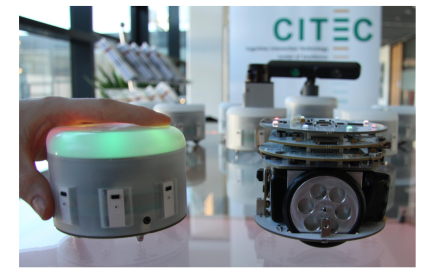
\includegraphics[width=\textwidth]{real_amiro_1}
    \caption{AMiRo with and without chassis \cite{AMiRo_paper_modular}.}
    \label{fig:real_1}
\end{figure}
\clearpage

\section{Hardware Architecture of AMiRo}
As mentioned in the previous chapter, the AMiRo is equipped with three basic board modules and two extension boards. In this section each board will be briefly discussed with a special emphasis in the functionalities that are of interest for this thesis. For a more complete discussion about the boards or the AMiRo in general, the reader is invited to read the documentation referenced in this work, specially \cite{AMiRo_paper_verstaile, AMiRo_paper_modular, AMiRo_paper_applications, AMiRo_ppt_v1, AMiRo_ppt_v2} whic\ can be found on the CITEC website or on the repository of this work on gitlab \cite{AMiRo_Git}.

The functionality of the sensors used in the project will be briefly explained in this chapter. For the explanation on how to read the output of the sensors that are sent via the Controller Area Network protocol, the reader is invited to jump directly into section \ref{sec:canconv} for reviewing the CAN convention used in the entire project and section \ref{sec:sensorout} for understanding each sensor's output.

In figure \ref{fig:schemat} a schematic of the AMiRo can be seen, with the three basic boards \textit{DiWheelDrive}, \textit{PowerManagement}, and \textit{LightRing} but also the extension boards \textit{ImageSensor}, \textit{Cognition}, and \textit{Image Processing}. The electrical interfaces are also displayed. For the current work, the most important thing to note in this image is that every board is able to talk to the CAN bus.

\begin{figure}[h]
	\centering
	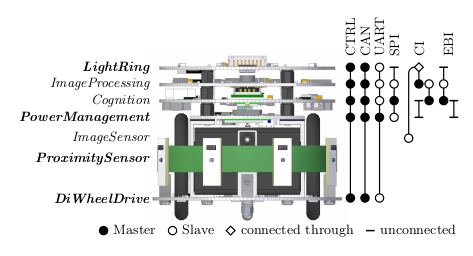
\includegraphics[width=\textwidth]{amiro_schematic}
    \caption{Inner parts of AMiRo with all extension boards, and overview of the electrical interfaces \cite{AMiRo_paper_modular}.}
    \label{fig:schemat}
\end{figure}
\clearpage

\subsection{DiWheelDrive}
\label{sub:DWD}
The DiWheelDrive is the bottom board of the AMiRo. It is equipped with an ARM Cortex-M3 based STM32F103 MCU from STMicroelectronics \cite{AMiRo_paper_modular}. It is through the DiWheelDrive's UART interface that the AMiRo's three basic modules get programmed. Each board gets programmed at a time with help of the AMiRo bootloader which will be discussed in section \ref{sub:btl}.

This board has two motors of 1W DC. The purpose of having two motors is to be able to have a differential kinematic to allow flexible movements \cite{AMiRo_paper_modular}. Among other sensors and actuators, the ones that are in this board and are being used in this thesis are: three axis gyroscope, accelerometer, and magnetometer, floor proximity sensors, the two motors, and optical motor encoders. The functionality and some specifications of the above mentioned sensors and actuators will be discussed in the next subsections.

As mentioned before, the DiWheelDrive board has a Cortex-M3 MCU for calculating such things as motion control, odometry, and dead reckoning algorithms at high sampling rates \cite{AMiRo_paper_modular}. This board can be accessed by the other boards via the Controller Area Network protocol or via USB UART interface directly with the user. It is important to mention that every board has also a USB UART interface to communicate directly with the user but all of them are covered by the chassis except for the DiWheelDrive board \cite{AMiRo_paper_modular}.

The \textit{DiWheelDrive} board ready to be mounted into the robot can be seen in figure \ref{fig:diwheel}. In this figure the board can be seen from both, top and bottom perspectives.

\begin{figure}[ht]
	\centering
	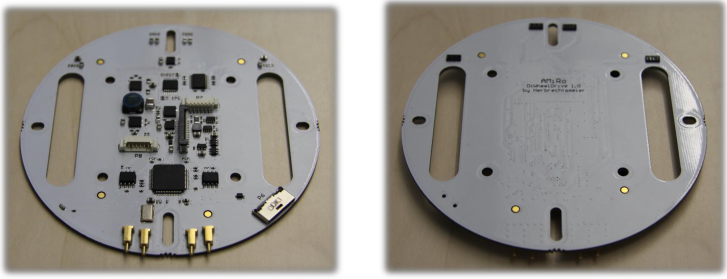
\includegraphics[width=\textwidth]{DiWheel_real}
    \caption{Top and bottom view respectively of the DiWheelDrive board \cite{AMiRo_ppt_v1}.}
    \label{fig:diwheel}
\end{figure}
\clearpage

\subsubsection{Gyroscope}
The gyroscope is a sensor that measures rotational motion. The units of the resulting measurement are revolutions per second or degrees per second. As a quick example, in a balancing robot a gyroscope can be used to measure how much the robot has rotated from the desired position and this information can be sent to an actuator to make corrections in order to reach the desired angle \cite{gyrostheory}. A gyroscope normally consists of a mass that moves with constant angular momentum, so when the gyroscope is tilted the axis of rotation of said mass reacts to the applied rotational movements making the axis of rotation tilt. This tilting leads to a displacement of the capacitance fingers inside the sensor which changes the capacitance. Finally when compared to a reference capacitance level, the angular velocity can be determined \cite{AMiRo_ppt_v1}.

The gyroscope used in the DiWheelDrive board is the l3g4200d from STMicroelectronics. This sensor communicates via SPI with the processor. This sensor is configured to have a resolution of $+/-500 dps$ in accordance with the user's manual \cite{gyroscopepart} and it is possible to obtain the output in degrees per second, micro degrees per second, revolutions per second, and micro revolutions per second with the current code. The actual units are degrees per second but the user can easily change the output selecting a different function from \textit{updateSensorVal()} function inside DiWheelDrive.cpp. For a more clear explanation on the code structure, see section \ref{AMiRo_OS}. The sensor communicates with the processor via SPI communication.

\subsubsection{Accelerometer}
The accelerometer is a sensor that measures the acceleration of an object. The units of the resulting measurement are meters per squared second or in g forces, where g as a unit equals $9.81 m/s^2$ \cite{accelerometertheory}. It is typically a system composed by a mass, a spring, and a damper. The mass moves according to the applied acceleration and changes the resulting capacitance that can be sent as an output for further reading and processing \cite{AMiRo_ppt_v1}.

The accelerometer used in the DiWheelDrive board is the lis331dlh from STMicroelectronics. This sensor is configured be scaled with a $+/-8g$ factor in accordance with the user's manual \cite{accelerometerpart}. The output is in g units and the sensor is being communicated via SPI with the processor.

\subsubsection{Magnetometer}
The magnetometer is a sensor that measures the magnetic field for all three physical axes \cite{magnetometertheory}. This sensor works thanks to three principles. The first one is called the \textit{Anisotropic magneto resistance effect} discovered in 1857 by William Thomson, in which an external magnetic field can make the sensor change the electrical resistance of a ferromagnetic material. The electrical resistance will be at a maximum value when the direction of the electrical current is parallel to said magnetic field \cite{AMiRo_ppt_v1}.

The second principle is called \textit{Fluxgate} and it is a way of calculate the vectorial measurement of a magnetic field invented by Friedrich Förster in 1937. The method starts with two cores wrapped by two coils of wire. There should be an electrical current driving the core through cycles of magnetic saturation. The resulting electrical current of the second coil will depend on the external magnetic field \cite{AMiRo_ppt_v1}.

The last principle is called the \textit{Hall effect} discovered in 1897 by Edwin Hall. In this principle can be visible when an electric current flows through a conductor in a magnetic field, the magnetic field will exert a transverse force on the moving charge carriers which tends to push them to one side of the conductor. The result is a voltage difference between both sides of the conductor \cite{halleffect}.

The magnetometer used in the DiWheelDrive board is the hmc5883l from STMicroelectronics. This sensor is configured to have a field resolution of $+/-5Gauss$ according to the user's manual \cite{magnetometerpart} and the current output is set to be in micro Gauss units. The sensor is being communicated via I2C protocol with the processor.

\subsubsection{Floor Proximity Sensor}
\label{sec:AMS}
The floor proximity sensor used is the "Fully Integrated Proximity and Ambient Light Sensor With Infrared Emitter", part vcnl4020 of Vishay \cite{proxsensor}. Four of these sensors are in the bottom of the AMiRo, programmed as light sensors, while other eight of these sensors are being used as proximity sensors and ambient light detectors coordinated by the Power Management board, see section \ref{PWB} for more information.

The ambient light sensor measures the intensity of light and its is measured in luminance. In order to do this the sensor usually consists of a photoresistor or a photo-sensitive material, outputting a resistance that can be measured and compared to a default value to estimate the luminance \cite{amstheory}.

The goal of providing AMiRo with these sensors attached to its bottom is to detect changes in the color of the floor. An example application can be for the AMiRo to follow a line or path painted on the ground, by making the robot recognize when it is over one color and when it is not.

\subsubsection{Motors}
As previously described in section \ref{sub:DWD}, the AMiRo has two DC motors of 1W each to offer a differential kinematic and to allow agile movements \cite{AMiRo_paper_modular}. These motors are connected to the DiWheelDrive board which means that this board controls the velocity of the motors and also knows the actual velocity of the motors.

The velocity of the motors can be set anytime from the Cognition board and the actual velocity of the AMiRo is one of the sensor values that can be asked from AMiRo's internal controller. The user can set and view the velocity in $\mu m/s$ or in $\mu rad/s$.

\subsubsection{Encoder}
AMiRo has optical encoders as well, that allow the user to know how much the motors have turned from a certain checkpoint. This data can be used to know how far the AMiRo has moved from a certain point. This sensor returns the $x$ coordinate in $\mu m$, the $y$ coordinate in $\mu m$, and the orientation of the wheels in $\mu rad$.

\subsection{Power Management}
\label{PWB}
The Power Management board is the central basic module of AMiRo. This board is responsible for the power supply and elementary behavior of the system. This is why it has the most powerful microcontroller. This board has an ARM Cortex-M4 based STM32F405 from STMicroelectronics. The characteristics from this microcontroller were needed to ensure a fast reaction times on critical system events and still provide enough headroom to additionally perform basic behaviors like obstacle avoidance, or homing \cite{AMiRo_paper_modular}.

There are two lithium-ion batteries connected to the Power Management board that power the whole system, and there are also some sensors on this board. Among the sensors that this board has, the ones that are being used by this project are: eight proximity sensors that act as proximity sensors and also as ambient light sensors, sensors for knowing if the charging cable is connected, the remaining battery charge or the time for a complete battery charge, the time for this both events to be completed, and the actual current consumption  \cite{AMiRo_paper_modular}.

The \textit{PowerManagement} board ready to be mounted into the robot can be seen in figure \ref{fig:powerm}. In this figure the board can be seen from both, top and bottom perspectives.

\begin{figure}[ht]
	\centering
	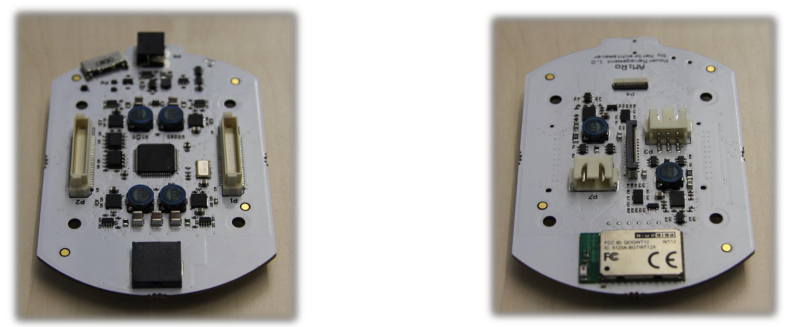
\includegraphics[width=\textwidth]{power_real}
    \caption{Top and bottom view respectively of the Power Management board \cite{AMiRo_ppt_v1}.}
    \label{fig:powerm}
\end{figure}
\clearpage

\subsubsection{Power Status}
For the tracking of the power status, AMiRo is equipped with a bq27500 Impedance Track from Texas Instruments that allows the robot to obtain information such as remaining battery capacity, state-of-charge, run-time to empty, battery voltage, and temperature \cite{impedancepart}.

\subsubsection{Proximity Ring}
As seen in section \ref{sec:AMS}, the eight vcnl4020 sensors in connected to the Power Management board are functioning as ambient light sensors and also as proximity sensors. For this last functionality, the sensor has a built-in infrared emitter and photo-pin-diode, having a maximum relying measurement of 200mm \cite{proxsensor}. These sensors are connected in a ring-fashion way so that the AMiRo has eight sensors throughout its entire circumference, making it able to detect obstacles in all horizontal directions. The units of the output are also in mm.

The \textit{Proximity Ring} ready to be mounted into the robot can be seen in figure \ref{fig:proxring}. The proximity ring gets attached to the \textit{Power Management} board as mentioned before.

\begin{figure}[ht]
	\centering
	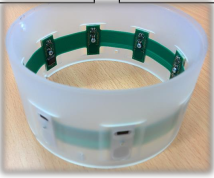
\includegraphics[]{prox_ring_real}
    \caption{Proximity Ring view \cite{AMiRo_ppt_v1}.}
    \label{fig:proxring}
\end{figure}
\clearpage

\subsection{Light Ring}
The Light Ring board is the top-most board in the AMiRo. This board has a STMicroelectronics ARM Cortex-M3 based STM32F103 MCU. It contains eight RGB LEDs arranged in a circular way corresponding to the Proximity Ring discussed in last section. The LEDs can be set from the Cognition board, setting each color of the RGB channels \cite{AMiRo_paper_modular}.

The \textit{LightRing} board ready to be mounted into the robot can be seen in figure \ref{fig:lightr}. In this figure the board can be seen from both, top and bottom perspectives. As it can be seen in the image, the LEDs are positioned equidistant in a circular fashion. This board is the upmost board which is covered by a translucent material, allowing the user to see the colors of the LEDs.

\begin{figure}[ht]
	\centering
	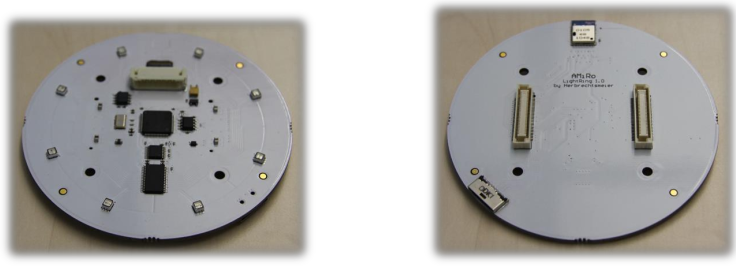
\includegraphics[width=\textwidth]{light_real}
    \caption{Top and bottom view respectively of the Light Ring board \cite{AMiRo_ppt_v1}.}
    \label{fig:lightr}
\end{figure}
\clearpage

\subsection{Cognition Board}
\label{sub:cogn}
This board was thought as an extension board which is no longer from the basic set of boards that make the AMiRo. The \textit{Cognition board} is being used as the Reflective Operator of the DA\_AMiRo project according to the OCM model. It provides the high-level functionality, gathering and coordinating the information via CAN that is generated in the three basic boards also known as the internal controller \cite{AMiRo_paper_modular}.

The most important feature of this board is the attached Gumstix Overo Computer-on-Module. In the current setup, the Overo TidalSTORM COM is being used, which combines an ARM Cortex-A8 based DaVinci DM3730 SoC from Texas Instruments \cite{AMiRo_paper_modular}. This board has the same serial programming port as on the three basic boards. Additionally, the board has also a Type A, a micro-AB, and an internal pin header USB interfaces \cite{AMiRo_paper_modular}.

The operating system running on the Overo COM is based on the Linux Yocto reference distribution Poky \cite{poky}, and the way it communicates with the three basic boards is through CAN, using a simple SocketCAN software-wrapper that is offered by this distribution \cite{AMiRo_paper_modular}.

The \textit{Cognition} board ready to be mounted into the robot can be seen in figure \ref{fig:cogb}. In this figure the board can be seen from both, the bottom and the top perspectives.

\begin{figure}[ht]
	\centering
	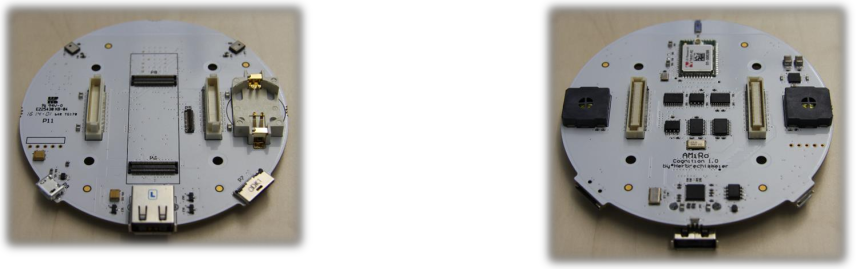
\includegraphics[width=\textwidth]{cognition_real}
    \caption{Bottom and top view respectively of the Cognition board \cite{AMiRo_ppt_v2}.}
    \label{fig:cogb}
\end{figure}
\clearpage

\section{Software Architecture of AMiRo OS}
\label{sec:soft}
As it has been discussed in previous sections, the AMiRo project was started back in 2015 and it is still being maintained. The version 1.0 of the project is the one from which this thesis is based on \cite{AMiRo_Git}.

\subsection{AMiRo bootloader}
\label{sub:btl}
The open-source bootloader for MCUs is the bootstrap for the three basic boards of the AMiRo. The AMiRo's bootloader is the responsible of configuring and setting up the computer for working with the AMiRo. The set-up that is provided in the bootloader is more than enough to successfully start working on the Operating System of AMiRo and programming it \cite{btl}.

As said before, the DiWheelDrive is the only module of which the programming port can be accessed by the user. This is why new software is applied to the two other basic boards by remote flashing via OpenBLT. Using CAN communication the new binary is forwarded by the DiWheelDrive board so that the target board receives the data and stores it in its flash memory \cite{AMiRo_paper_modular}.

\subsection{AMiRo real-time operating system kernel}
The real-time operating system that is being used is the open-source ChibiOS. This project aims at creating a portable, light weight, and fast real-time operating system for embedded applications \cite{chibioshp}. ChibiOS not only provides low-level drivers for all interfaces of the most common microcontrollers, but it also gives an unified hardware abstraction layer, priority based preemptive scheduling, and high-performance event and message passing systems. ChibiOS can be configured statically and dynamically to exactly fit the application in order to maximize efficiency and performance \cite{AMiRo_paper_modular}.

\subsubsection{ChibiOS}
Some of the main characteristics from ChibiOS are:

\begin{itemize}
\item System time: ChibiOS has a 16 or 32 bits system time counter.
\item Real tick-less mode: There is no periodic system tick for optimal power management.
\item IRQ Management: ISRs abstraction.
\item Preemption: Fully preemptive scheduling.
\item Round robin scheduling: Round robin scheduling for threads at equal priority.
\item Messages: Inter-thread synchronous messages.
\item Mailboxes: Message queues.
\item Counter semaphores: Semaphores with boolean state.
\item Binary semaphores: Semaphores with boolean state.
\item Mutexes: Mutexes implementing the priority inheritance algorithm.
\item Events: Events, event flags, event sources.
\item Dynamic services: Dynamic threading.
\end{itemize}

Note: All the above mentioned characteristics can be found and further explained in the ChibiOS homepage. \cite{chibioshp}

A project containing ChibiOS consists on the Operating System source files, few configuration files and a HAL file for the peripherals handling.

\subsection{AMiRo Operating System structure}
\label{AMiRo_OS}
AMiRo's Operating System or board specific abstraction layer from the original repository \cite{AMiRo_Wiki} includes two basic applications, the first one is a rudimentary command shell and the second one a hardware test. The first one is already integrated in ChibiOS and it is extended by module specific commands \cite{AMiRo_paper_modular}.

The structure of the AMiRo Operating System, including the files that are being used with the current project can be visualized in figure \ref{fig:OS}. The entire project is written in C++ language, with some inclusions of C code. In this figure, it can be seen that inside \textit{AMiRo\_OS} there is the \textit{components} folder which contains the shared codes that the three boards are using. The other part of the structure worth mentioning now is the \textit{devices} folder in which the three boards have their own set of files, always maintaining the same structure among them.

\begin{figure}[ht]
	\centering
	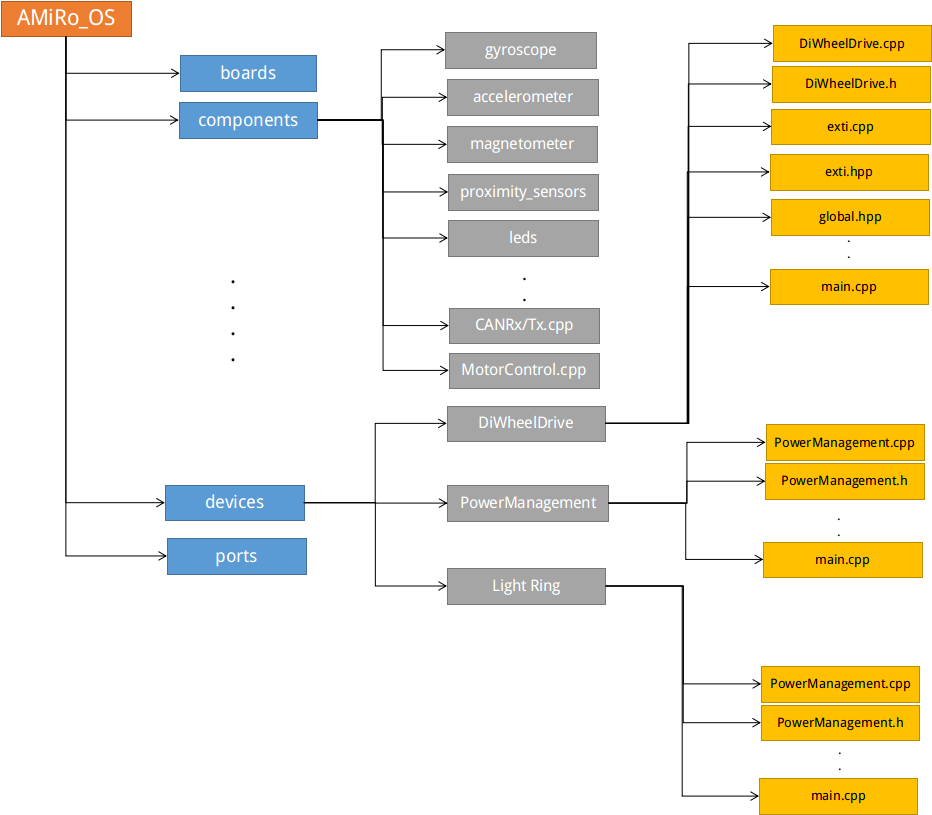
\includegraphics[width=\textwidth]{AMiRo_OS}
    \caption{AMiRo\_OS breakdown structure}
    \label{fig:OS}
\end{figure}

\subsection{AMiRo Operating System functionality}
As mentioned before, the AMiRo OS has a command shell application which has a set of pre-stablished commands corresponding to commands that can set the lights of the AMiRo on, the motors, calibrate sensors, set a desired velocity or a distance for AMiRo to travel, get some sensor values, among other things.

There are two parent classes for all of the three basic boards: ControllerAreaNetworkTx.cpp and ControllerAreaNetworkRx.cpp. The ControllerAreaNetworkTx.cpp has the following functions:

\begin{itemize}
\item setLightBrightness(int brightness)
\item setLightColor(int index, Color color)
\item setOdometry(types::position robotPosition)
\item setTargetSpeed(int32\_t leftURpm, int32\_t rightURpm)
\item setTargetSpeed(kinematic \&targetSpeed)
\item setTargetPosition(types::position \&targetPosition, uint32\_t targetTime)
\item setKinematicConstants(float Ed, float Eb)
\item broadcastShutdown()
\item txQueryShell(uint8\_t toBoardId, char *textdata, uint16\_t size)
\item txReplyShell(uint8\_t toBoardId, char *textdata, uint16\_t size)
\item main(void)
\item updateSensorVal()
\item encodeBoardId(CANTxFrame *frame, int board)
\item encodeDeviceId(CANTxFrame *frame, int device)
\item encodeIndexId(CANTxFrame *frame, int index)
\item transmitMessage(CANTxFrame *frame)
\end{itemize}

Among these functions, it can be seen that the ControllerAreaNetworkTx.cpp is the responsible for updating the sensor values and for broadcasting them. Another feature of this class is to manage the outgoing CAN frames, coding the device id, the board id and also the id of the index from the commands.

The ControllerAreaNetworkRx.cpp is the responsible of managing the incoming CAN frames and the functions of this class are:

\begin{itemize}
\item getProximityRingValue(int index)
\item getProximityFloorValue(int index)
\item getActualSpeed(types::kinematic \&targetSpeed)
\item getOdometry()
\item getPowerStatus()
\item getRobotID()
\item getMagnetometerValue(int axis)
\item getGyroscopeValue(int axis)
\item calibrateProximityRingValues()
\item calibrateProximityFloorValues()
\item rxCmdShell(CANRxFrame *frame)
\item main(void)
\item decodeBoardId(CANRxFrame *frame)
\item decodeDeviceId(CANRxFrame *frame)
\item decodeIndexId(CANRxFrame *frame)
\item receiveSensorVal(CANRxFrame *frame)
\end{itemize}

From the shown functions in ControllerAreaNetworkRx.cpp it is clear that this class receives the CAN frames, decodes the board, index, and device information. Once the purpose of the incoming CAN frame has been found out, the ControllerAreaNetworkRx.cpp proceeds to make use of the CAN frame according to its topic, if for example the CAN frame wanted to set the robot's position, the CANRx.cpp will set the values of robotPosition.x, robotPosition.y, and so on with the content of said frame. From the names of the functions, the reader can have a broad idea from what each of them does with the received CAN frame.

Now that the functionality of the CANRx/Tx.cpp has been shown, each one of the three boards that inherit from them will be briefly discussed.

\subsubsection{DiWheelDrive project}
Lets look at \textit{main.cpp} from \textit{DiWheelDrive} board. The shell which was already mentioned is being managed by this board. Every sensor that will be used is waken up and the communications protocols for each one is started. It is also in this code where all the threads are being started. The threads are:

\begin{itemize}
  \item Power status
  \item Magnetometer
	\item Gyroscope
	\item Accelerometer
	\item Proximity floor sensors
	\item Motor control
	\item Odometry
	\item User thread
\end{itemize}

Each one of these threads is also a class which objects are created in the \textit{global.hpp} so that the encapsulated values of each object can be accessed from the outside. In global.h all the sensors corresponding to the \textit{DiWheelDrive} are initialized and configured for its use. As an example, the registers for using the magnetometer or \textit{hmc5883l} are configured to set the number of samples averaged, select the data output rate bits, set the measurement configuration bits, set the gain configuration bits, among other things. For more precise information about the registers and how to configure the sensors, please refer to the sensor's data sheet, in this case \cite{magnetometerpart}.

Global is also a class and an instance of it is created in \textit{main.cpp} which is called \textit{robot}, meaning that from \textit{main.cpp} the user can access the elements of \textit{robot} among which are the instances of the sensors listed above. For example, in order to access the magnetometer, the user has to use something like this: \textit{robot.hmc5883l...}.

Regarding the threads listed above, the Power status in this board only makes a self test and initiates a power monitor. The magnetometer, gyroscope, accelerometer, power status, odometry, and the proximity floor classes, have functions for updating their sensor's data, and functions for getting the actual sensor's value in a raw format and also with a specific unit. For the available units for every sensor, see section \ref{sub:sensors}.

The threads of the magnetometer, gyroscope, accelerometer, power status, odometry, and proximity floor sensors are constantly updating their values so that they are ready whenever they are required. As a side note, the magnetometer thread, the gyroscope thread, the accelerometer thread, and the proximity floor sensors thread are constantly broadcasting to the CAN bus at a given frequency which is set to $16Hz$.

The motor control thread is constantly updating the increments of velocity, the speed, calculating velocities in desired units. In addition to this, the thread updates past velocities for the derivative part of a PID controller tje user has access to, and writes the calculated duty cycle of the PWM driver.

Lastly, the user thread of the \textit{DiWheelDrive} is a complete line following application that makes AMiRo able to follow a black line on the ground that is over a white surface.

The overall structure from the \textit{DiWheelDrive} project can be seen in figure \ref{fig:DWDclassOS} where the sensors are broadcasting their values at once to the CAN bus. Also, as discussed before, the ControllerAreaNetworkRx.cpp is constantly monitoring the CAN bus for commands that would like to calibrate or select a desired end value in the encoders and the motors, but also for controlling the motors themselves.

\begin{figure}[ht]
	\centering
	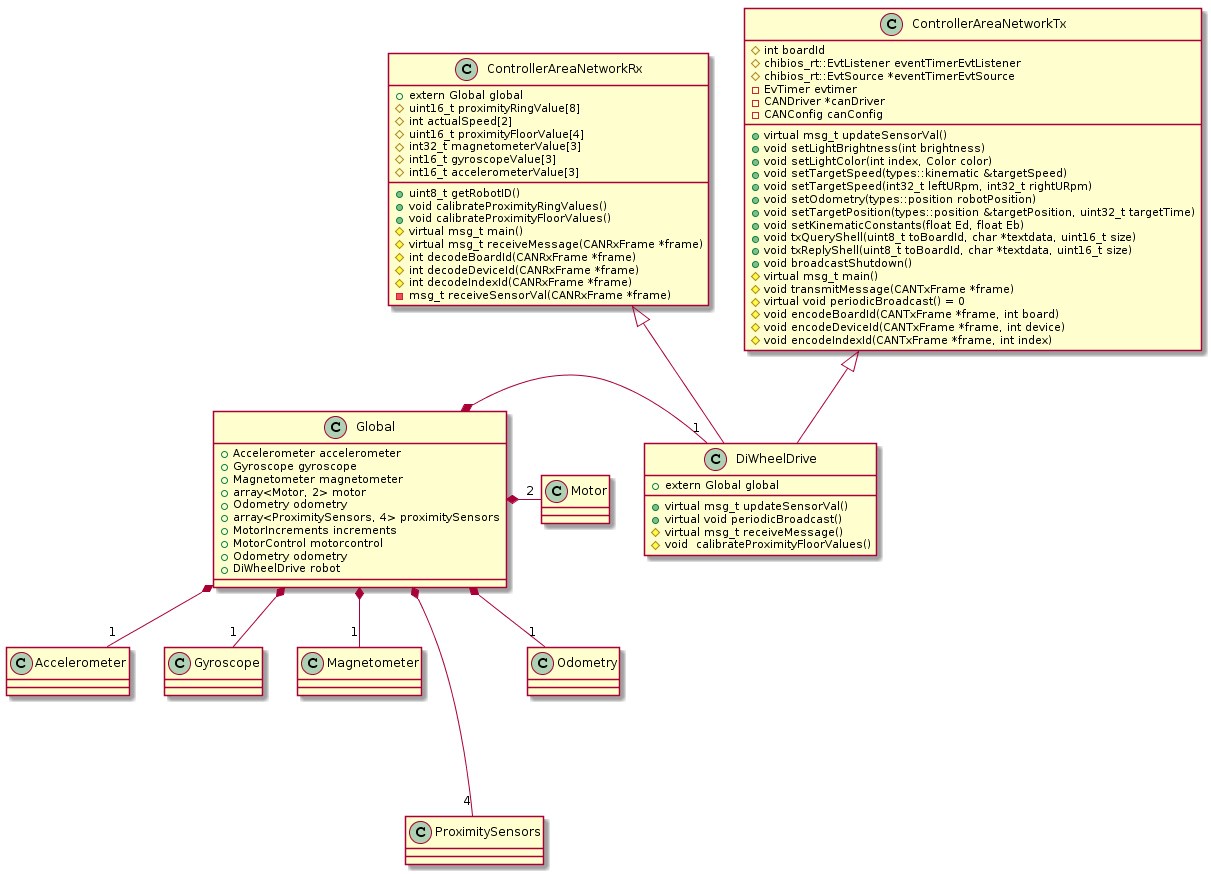
\includegraphics[width=\textwidth]{DWDclass_OS}
    \caption{DiWheelDrive broad class diagram of AMiRo OS}
    \label{fig:DWDclassOS}
\end{figure}

\subsubsection{Power Management project}
The \textit{Power Management} project follows the same structure mentioned for the \textit{DiWheelDrive}, with a \textit{main.cpp} and its own \textit{global.hpp}. The instance of the global class is also called \textit{robot} and also can be accessed from the \textit{main.cpp}. The list of the threads of the \textit{Power Management} is as follows:

\begin{itemize}
  \item Power status
	\item Proximity ring sensors
	\item ADC
	\item Touch sensors %mpr121 part of the ring sensors
	\item User thread
\end{itemize}

The proximity ring and the touch sensor threads are constantly updating its sensors' values. The touch sensor \textit{mpr121} is part of the proximity ring sensors structure and these two sensors are also broadcasting its values through the CAN bus like the ones from \textit{DiWheelDrive}.

The power status thread receives help of the ADC thread which constantly monitoring the charge of the batteries and converting the analog levels of charge to a digital number. The power status thread then it is frequently updating values such as the current battery levels, the time of charge remaining, whether or not AMiRo is plugged in, and the current consumption.

The user thread of the \textit{Power Management} is an obstacle avoidance application for the AMiRo which also sends commands via CAN to the \textit{DiWheelDrive} in order to stop the AMiRo or stir it in order to stop it from crashing.

The overall structure from the \textit{PowerManagement} project can be seen in figure \ref{fig:PMclassOS} where the sensors are broadcasting their values at once to the CAN bus. Also, as discussed before, the ControllerAreaNetworkRx.cpp is constantly monitoring the CAN bus for commands that would like to calibrate the proximity ring sensors.

\begin{figure}[ht]
	\centering
	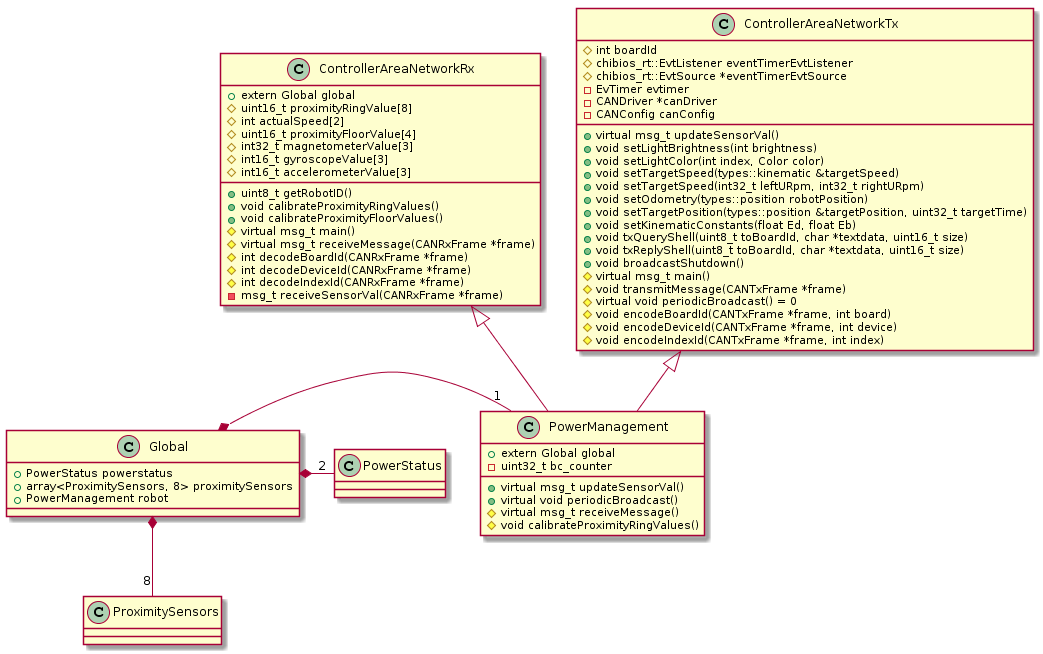
\includegraphics[width=\textwidth]{PMclass_OS}
    \caption{PowerManagement broad class diagram of AMiRo OS}
    \label{fig:PMclassOS}
\end{figure}

\subsubsection{Light Ring project}
Finally the \textit{Light Ring} project is the simplest of the three projects, it follows the same structure mentioned for the \textit{DiWheelDrive} and \textit{Power Management}, with a \textit{main.cpp} and its own \textit{global.hpp}. The instance of the global class is also called \textit{robot} and also can be accessed from the \textit{main.cpp}. The list of the threads of the \textit{Light Ring} is as follows:

\begin{itemize}
	\item Lidar
	\item LEDs
	\item User thread
\end{itemize}

The lidar thread is performing a configuration of the lidar and a quick check to see if it is communicating correctly with the system. Afterwards it is constantly updating its values.

The LEDs thread is constantly refreshing the LEDS with the preset brightness values and the colors assigned to each of them.

The user thread of the \textit{Light Ring} has no implemented application and remains open for the user to assign one.

The overall structure from the \textit{LightRing} project can be seen in figure \ref{fig:LRclassOS} where the sensors are broadcasting their values at once to the CAN bus. Also, as discussed before, the ControllerAreaNetworkRx.cpp is constantly monitoring the CAN bus for commands that would like to set the LEDs to a certain color and to adjust the brightness.

\begin{figure}[ht]
	\centering
	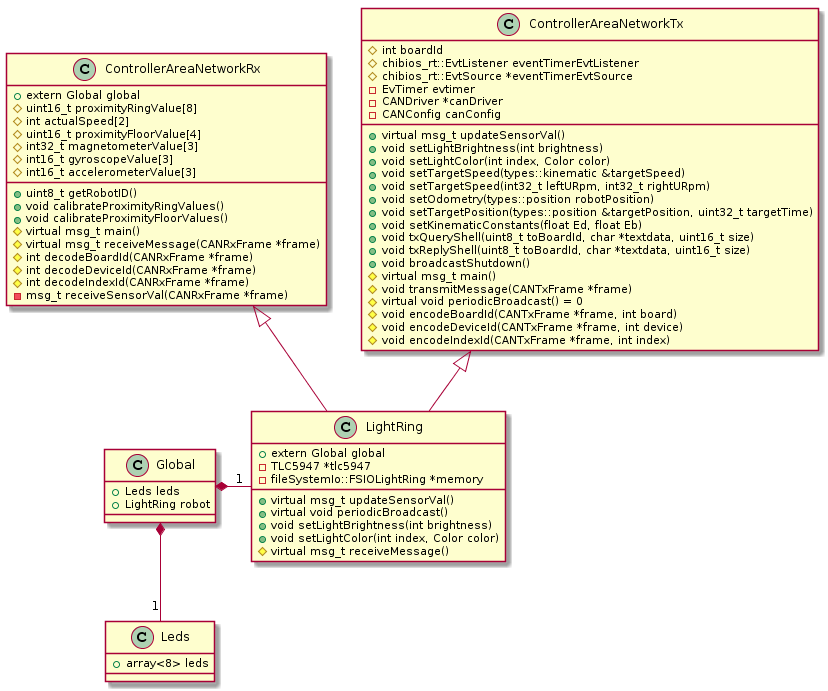
\includegraphics[width=\textwidth]{LRclass_OS}
    \caption{LightRing broad class diagram of AMiRo OS}
    \label{fig:LRclassOS}
\end{figure}

%\clearpage
\chapter{DA\_AMiRo software architecture}
From the past chapter the hardware and software structure of the AMiRo was mentioned and discussed. From this point forward the structure and functionality of the DA\_AMiRo project which is based on the OCM model will be discussed as it is the central point of the master thesis. As a friendly reminder, the reader can obtain the source codes made for the DA\_AMiRo project from the repository \cite{AMiRo_Git}.

\section{DA\_AMiRo software structure}
In last chapter, the AMiRo's Operating System structure was introduced. This Operating System is the one located on top of figure \ref{fig:DAAMIROstr}, inside the folder called \textit{amiro\_1.0\_stable}. In order to fulfill the requirements of the DA\_AMiRo project, the AMiRo OS had to be changed for a OCM apporach, and the functionality of the resulting software structure will be discussed in section \ref{sub:DAAMIROOS}.

\begin{figure}[ht]
	\centering
	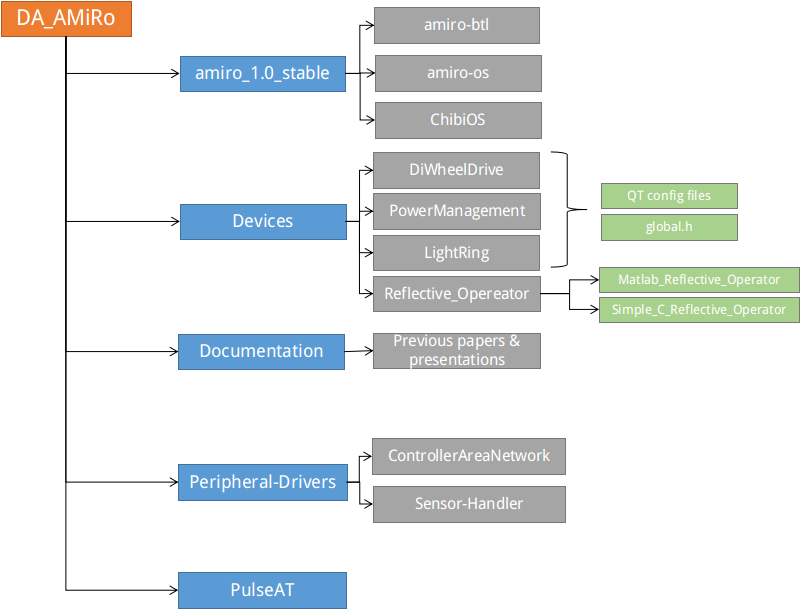
\includegraphics[width=\textwidth, height=13cm]{DAAMIRO}
    \caption{DA\_AMiRo overall structure}
    \label{fig:DAAMIROstr}
\end{figure}

The configuration files for the three projects are located inside the \textit{Devices} folder which can be visualized in figure \ref{fig:DAAMIROstr}. They configure the QT IDE for each of the three boards, so the user can easily code and create the binary to program the AMiRo's boards. It is also inside this folder where the \textit{Reflective Operator} is located. The Reflective Operator consists of three parts: a simple C application, a Matlab application for the MuRoX board where a Simulink model that can be programmed into the Reflective Operator is located, and four already compiled and functioning Demo Applications. These Demo Applications will be discussed in chapter \ref{chap:reflective}, but it is worth mentioning that they are already inside the MuRoX board, ready to be used.

Inside the \textit{Peripheral-Drivers} the user can find the ControllerAreaNetwork.h responsible of having the structures and all the definitions that are being used by both the Internal Controller corresponding to the three basic boards and the \textit{Reflective Operator} which is being done by the MuRoX board. It is also inside this folder that the \textit{sensorhandler.cpp} and \textit{sensorhandler.h} are found. These both files manage the scheduling of the sensor data and they will be discussed in chapter \ref{chap:sensorDH}.

Finally, the folder \textit{Documentation} has some of the papers and information that the AMiRo has had since it was created. The reader can go inside this folder for getting more information about the AMiRo. In the other hand, the folder \textit{PusleAT} was created for a future usage and it is still a work in progress.

\section{DA\_AMiRo Operating System's functionality}
\label{sub:DAAMIROOS}
In this section, the functionality of the DA\_AMiRo Operating System from figure \ref{fig:OS} will be addressed.

The DiWheelDrive board, the DiWheelDrive class inherits from both ControllerAreaNetworkRx.cpp and from ControllerAreaNetworkTx.cpp, making it capable of sending and receiving CAN frames. This happens exactly the same in the three boards. The CAN frame structure will be further discussed in chapter \ref{chap:CAN}. The DiWheelDrive class also implements the functions for updating each of the sensor's values and sending independently the data via CAN interface. As it can be seen in figures \ref{fig:DWDclass}, \ref{fig:PMclass}, and \ref{fig:LRclass}, DiWheelDrive has virtual functions of every sensor including the Power Management board and also the Light Ring board. These functions however, have a '= 0' which means that they are not being implemented in this specific class. Similarly in the other two boards the same thing happens with their own set of sensors.

This means that in the DiWheelDrive class, the functions that are being implemented correspond to the gyroscope, accelerometer, magnetometer, proximity sensors, motors, and encoders. In the Power Management class the implemented functions include proximity sensors and power status sensors, and in the Light Ring class the implemented function concerns only the LEDs for the purposes of DA\_AMiRo.

The global class is the responsible for creating each object from each sensor and encapsulating them under the name of 'robot'. This makes the \textit{robot's} attributes accessible from other classes. This means that, for example, the gyroscope's value can be updated and outputted as a part of \textit{robot} from other parts of the code. The global object is finally initialized in the main function, as well as the threads responsible for managing the scheduler of the sensor's data but this subject will be discussed more deeply in chapter \ref{chap:sensorDH}.

\begin{figure}[ht]
	\centering
	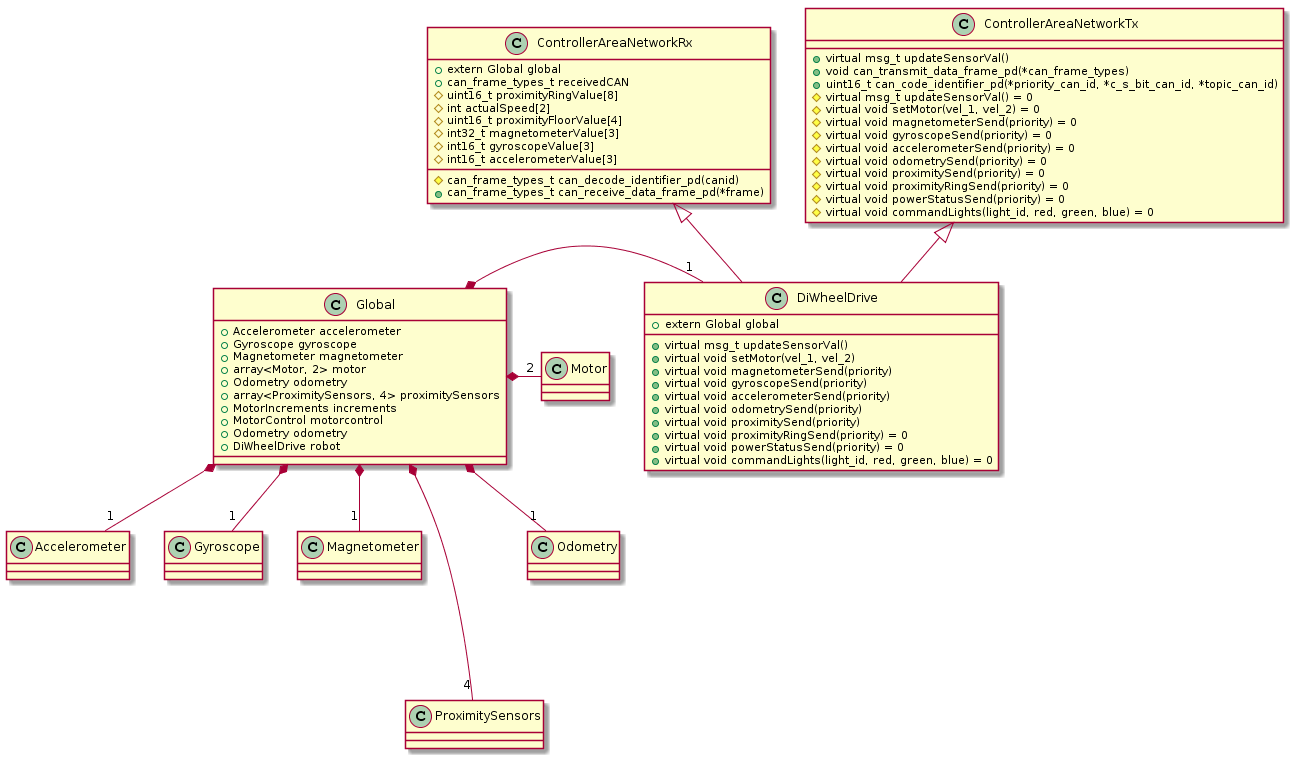
\includegraphics[width=\textwidth]{DWDclass}
    \caption{DiWheelDrive broad class diagram}
    \label{fig:DWDclass}
\end{figure}

\begin{figure}[ht]
	\centering
	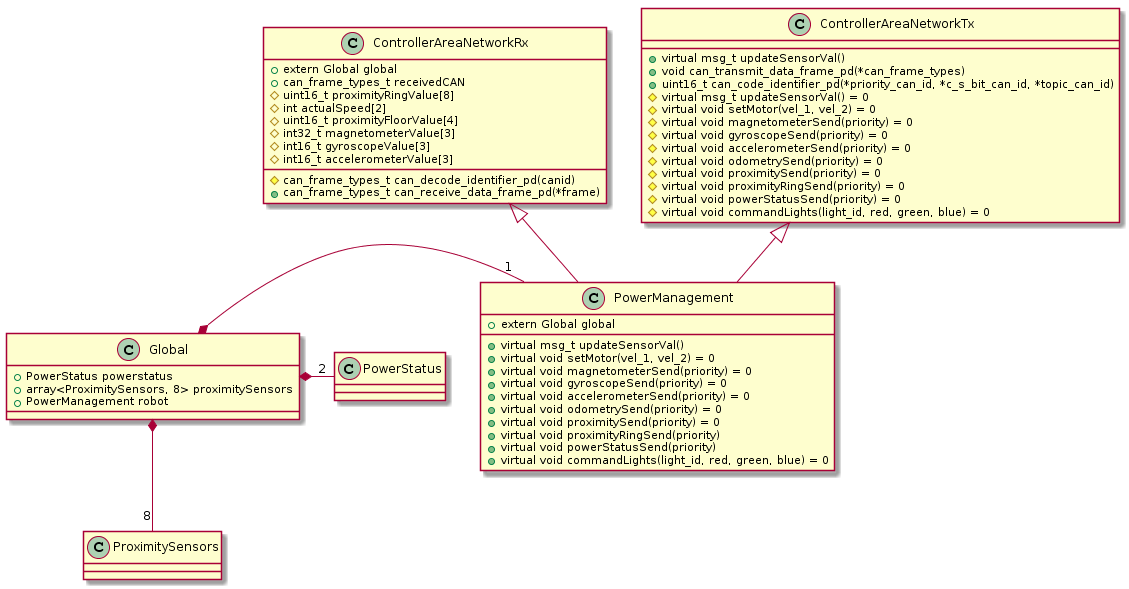
\includegraphics[width=\textwidth]{PMclass}
    \caption{PowerManagement broad class diagram}
    \label{fig:PMclass}
\end{figure}

\begin{figure}[ht]
	\centering
	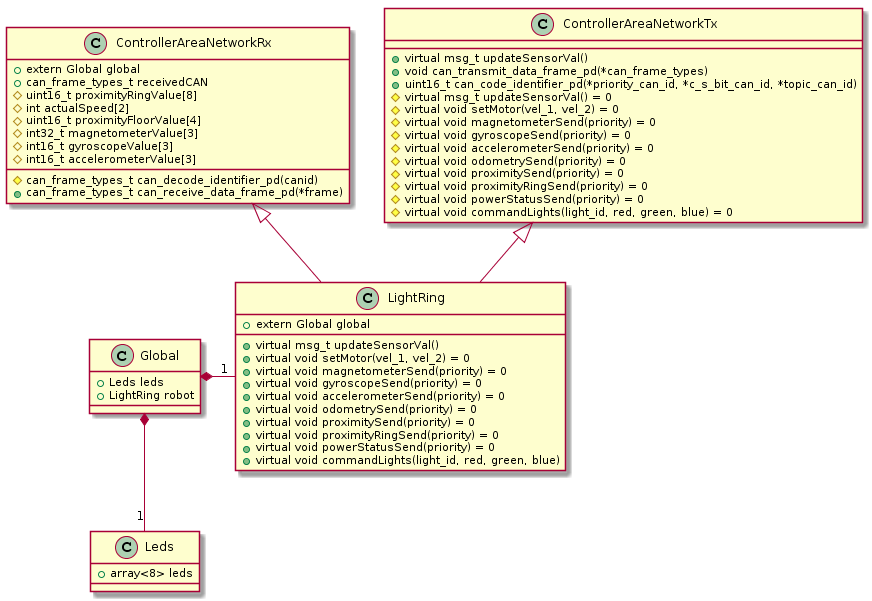
\includegraphics[width=\textwidth]{LRclass}
    \caption{LightRing broad class diagram}
    \label{fig:LRclass}
\end{figure}

\chapter{Controller Area Network}
\label{chap:CAN}
This chapter explains how to receive and transmit CAN frames in the AMiRo. The functionality of the CAN module had to be merged with the current ControllerAreaNetworkRx.cpp and ControllerAreaNetworkTx.cpp of the existing repository of AMiRo \cite{AMiRo_Wiki}. The ControllerAreaNetwork.h however, is the same for the internal controller and for the \textit{Reflective Operator}. The reason behind sharing the ControllerAreaNetwork.h among projects is to be able to use a single set of definitions for names of sensors and some structures.

For starters, the baud rate requirement of the DA\_AMiRo project was set to 500kHz This frequency was achieved with the following equation, and can be changed from the CANRx and CANtx.cpp files that can be located with help of figure \ref{fig:OS}.

\begin{equation} \label{eq:baudrate1}
	500kHz= \frac{8MHz}{(B1+B2+SW)*prescaler}
\end{equation}

Where the 8MHz is the clock frequency of the STM32F3, the B1 and B2 are the time quanta bit segment one and two accordingly. Finally, the SW represents the maximum time quanta. These values were configured by the previous AMiRo project which also happened to configure the CAN frequency to 500kHz. The values and the names of the variables in the actual code are: $$B1 = CAN\_BTR\_TS1 = 13$$ $$B2 = CAN\_BTR\_TS2 = 2$$ and $$SW = CAN\_BTR\_SJW = 1$$ $$Prescaler = CAN\_BTR\_BRP = 1$$, which results in the following equation:

\begin{equation} \label{eq:baudrate2}
	\frac{8MHz}{(13+2+1)*1} = 500kHz
\end{equation}

\section{Convention used for sending and receiving frames}
\label{sec:canconv}

The format of the CAN frames was done accordingly with the pre-established convention for the DAEbot project \cite{DAEbot_Wiki} by Uwe Jahn. The format of the standard id from a CAN frame can be seen in figure \ref{fig:can}, where it is basically divided into three main parts. The command or sensor bit is the bit that allows devices on the CAN bus to know if the frame belongs to a command, i.e. knowing the value 'x' axis of the gyroscope, or setting the LEDs to red, or if it belongs to a sensor frame, i.e. the actual value of the 'x' axis of the gyroscope.

The second part is the priority which allows the devices on the bus know the priority of the command or sensor. If there are two frames in the bus at the same time asking for a sensor value from the same board for example, the priority will allow the system to preempt the frame of the one with higher priority.

The third and last part of the id from the frame is the topic id. The list for the topics can be seen in the ControllerAreaNetwork.h shared by all the devices or also from the ods file inside the same path \textit{Peripheral-Drivers/ControllerAreaNetwork/} from figure \ref{fig:DAAMIROstr}.

\begin{figure}[ht]
	\centering
	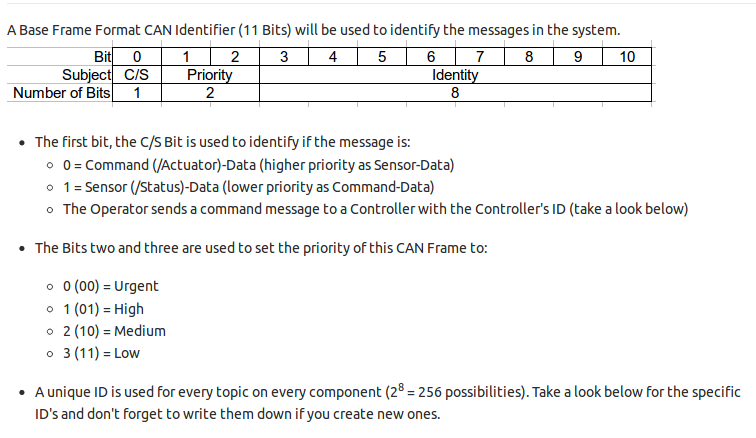
\includegraphics[width=\textwidth]{can_structure}
    \caption{Pre-established CAN frame format \cite{DAEbot_Wiki}}
    \label{fig:can}
\end{figure}

For the transmission of a CAN frame, the id is coded according to figure \ref{fig:can} and when a CAN frame is received, the id is decoded into the same structure. The CAN frame pre-established structure can be seen in snip of code \ref{CAN:frame}, which can be compared with the figure \ref{fig:can}. In this structure the only thing that has not been yet discussed is the data itself. The dlc is the number of bytes to be transmitted and the information is stored in the data8, data16 and data32 arrays. Thanks to the \textit{union} of these arrays, the same value can be accessed in different bit sizes.

\begin{minipage}{\linewidth}
\begin{lstlisting}[caption = CAN frame, label = CAN:frame, language = C, captionpos = b]
typedef struct can_frame_types {
    priority_can_id_t priority_id;
    c_s_bit_can_id_t c_s_bit_id;
    topic_can_id_t topic_id;
    uint8_t dlc;
    union{
        uint8_t     data8[8];
        uint16_t    data16[4];
        uint32_t    data32[2];
    };
} can_frame_types_t;
\end{lstlisting}
\end{minipage}

In order to send a CAN frame, can\_transmit\_data\_frame\_pd(...) can be called. When sending a CAN frame, the id is set to be in standard mode. The CAN frame that is sent consists of three main parts: id, DLC, and the data. The id is therefore set with the can\_code\_identifier\_pd(...) function before actually calling the transmit function. This function combines the c\_s bit with the priority bit and then combines that value to the topic ID. The CAN frame is later sent through the CAN driver.

On the CAN reception side, the status of the reception is assigned when calling to the can\_receive\_data\_frame\_pd(...) function. The status of the CAN reception can be successful, timeout, or error. Then the id of the CAN frame gets decoded with the function can\_decode\_identifier\_pd(...) and the data frames are passed into a global structure like in snip of code \ref{CAN:frame}

Note that can\_code\_identifier\_pd(...) and can\_decode\_identifier\_pd(...) are functions that were already implemented beforehand, for this project it was necessary to adjust both functions to operate with the current hardware platform.

%\clearpage
\section{Interpreting CAN frames of the sensors}
\label{sec:sensorout}
In this section it will be explained how to read the frames corresponding to each sensor. For the same reason, this section is divided into two subsections: sensors and actuators.

\subsection{Sensors}
\label{sub:sensors}
In order to interact with a sensor, the id from the CAN frame's command has to obey the convention shown in figure \ref{fig:can} and its content, the actual data from the CAN frame has to follow the convention shown in figure  \ref{fig:sensormodes} created for the DAEbot project.

There are three ways or modes in which a command can ask for data from a sensor. The first one is the mode one which asks for a sensor's data with a specific frequency. The first DLC of the CAN frame has to be set to '1' to activate the publisher mode. The second and third DLCs specify the numeric value of the frequency in format of little-endian. This means that the most significant bit should be a part of the DLC number 2 and the less significant bit should be a part of the DLC number 1. The fourth DLC specify the units of the value given in the second and third DLCs. This value can be obtained looking at figure \ref{fig:sensormodes}.

\begin{figure}[ht]
	\centering
	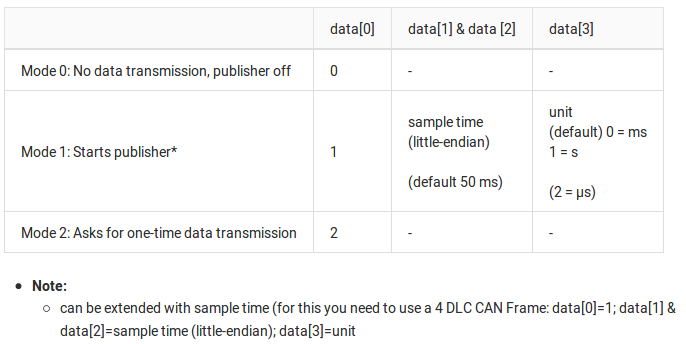
\includegraphics[width=\textwidth]{modes}
    \caption{Pre-established CAN modes for transmitting sensor data \cite{DAEbot_Wiki}}
    \label{fig:sensormodes}
\end{figure}

For example for starting publisher of the magnetometer 'x' axis, with normal priority, the CAN id should be composed by:

\begin{itemize}
	\item C\_S bit set to '0' on binary
	\item Priority set to '10' on binary
	\item Topic id of the gyroscope 'x' axis '0x05' on hexadecimal
\end{itemize}

So a value equal of '01000000101' in binary or '0x205' in hexadecimal. Now lets say we want the magnetometer 'x' axis value every $900\mu s$. The value '900' in decimal is '0x0384' in hexadecimal, making the little-endian adjustment for the bytes will result in '8403'. $\mu s$ is equal to '0x02'.

As a result, the complete CAN frame is: '0x205' for the id, '4' for the DLC or Data Length Code, each with the following values:

\begin{itemize}
	\item DLC 0: 0x01
	\item DLC 1: 0x84
	\item DLC 2: 0x03
	\item DLC 3: 0x02
\end{itemize}

This command would trigger the DiWheelDrive to output the magnetometer 'x' axis value every $900\mu s$, with an id that is almost the same but with the C\_S bit set to '1' instead, so that the CAN bus knows that this frame belongs to a sensor data. The topic id then will be '0x605' instead of '0x205'. The way of reading and understanding the outputted value for each sensor will be mentioned in the following subsections.

The second mode is the \textit{One-time data transmission} and it will only return the required sensor value one time. For the example of a one time transmission of the floor proximity sensors, the id of the CAN frame should be '0x204' with DLC 0: 2.

The third mode is the mode '0' which actually stops an on-going publishing of a sensor value given the frame's id. This means that in the example used for the explanation of mode '1' the way of stopping the transmission of the magnetometer 'x' axis, the id of the CAN frame should be the same '0x205', with DLC 0: 0.

\subsubsection{Gyroscope}
The three axis of the gyroscope come together in one CAN frame with a DLC of six. Each value has a size of 16bits with a format  of little-endian. Every value comes in two's complement and the units are degrees per second, and the resolution is $+/-500 dps$. See table \ref{tab:gyroscope}.

\begin{table}[h!]
\centering
\begin{tabular}{|l|l|}
	\hline
	DLC						&	6													\\	\hline
	size of data	&	16bits										\\	\hline
	'x' axis			&	DLC[1] DLC[0]							\\	\hline
	'y'	axis			&	DLC[3] DLC[2]							\\	\hline
	'z'	axis			&	DLC[5] DLC[4]							\\	\hline
	units					&	dps												\\	\hline
	note					& value in two's complement \\	\hline
\end{tabular}
\caption{\label{tab:gyroscope} CAN frame format from the output of the gyroscope}
\end{table}

\subsubsection{Accelerometer}
The three axis of the accelerometer come together in one CAN frame with a DLC of six as the gyroscope. Each value has a size of 16bits with a format of little-endian. Every value comes in two's complement and the units are $mili g$, and the result is scaled $+/-8g$. See table \ref{tab:accelerometer}.

\begin{table}[h!]
\centering
\begin{tabular}{|l|l|}
	\hline
	DLC						&	6													\\	\hline
	size of data	&	16bits										\\	\hline
	'x' axis			&	DLC[1] DLC[0]							\\	\hline
	'y'	axis			&	DLC[3] DLC[2]							\\	\hline
	'z'	axis			&	DLC[5] DLC[4]							\\	\hline
	units					&	$mili g$									\\	\hline
	note					& value in two's complement \\	\hline
\end{tabular}
\caption{\label{tab:accelerometer} CAN frame format from the output of the accelerometer}
\end{table}

\subsubsection{Magnetometer}
In the case of the Magnetometer, every axis has an independent id, this is because the size of the data is 32bits in little-endian format. Every value comes in two's complement and the units are $\mu Gauss$, and the result is scaled by $+/-5Ga$. See table \ref{tab:magnetometer}.

\begin{table}[h!]
\centering
\begin{tabular}{|l|l|}
	\hline
	DLC						&	4														\\	\hline
	size of data	&	32bits											\\	\hline
	'x' axis			&	DLC[3] DLC[2] DLC[1] DLC[0]	\\	\hline
	'y'	axis			&	DLC[3] DLC[2] DLC[1] DLC[0]	\\	\hline
	'z'	axis			&	DLC[3] DLC[2] DLC[1] DLC[0]	\\	\hline
	units					&	$\mu Gauss$									\\	\hline
	note					& value in two's complement 	\\	\hline
\end{tabular}
\caption{\label{tab:magnetometer} CAN frame format from the output of the magnetometer}
\end{table}

\subsubsection{Floor proximity sensors}
The four proximity sensors on the bottom of the AMiRo are together in one CAN frame with a DLC of eight. Each value has a size of 16bits with a format of little-endian. The data is in luminance with units candelas per squared meter $cd/m^2$. See table \ref{tab:floorprox} and note that this sensor does not return a two's complement value.

\begin{table}[h!]
\centering
\begin{tabular}{|l|l|}
	\hline
	DLC						&	8													\\	\hline
	size of data	&	16bits										\\	\hline
	sensor 1			&	DLC[1] DLC[0]							\\	\hline
  sensor 2			&	DLC[3] DLC[2]							\\	\hline
	sensor 3			&	DLC[5] DLC[4]							\\	\hline
	sensor 4			&	DLC[7] DLC[6]							\\	\hline
	units					&	$cd/m^2$									\\	\hline
\end{tabular}
\caption{\label{tab:floorprox} CAN frame format from the output of the floor proximity sensors}
\end{table}

\subsubsection{Encoder}
This sensor returns both the actual velocity and the odometry of the AMiRo. The first value will be the actual velocity followed by the odometry. For the odometry, the 'x' coordinate in $\mu m$ with a size of 32bits, the 'y' coordinate in $\mu m$ with a size of 32bits with a format of little-endian, and the orientation of the wheels in $\mu rad$ with a size of 16bits. All of these values are together in one CAN frame. See table \ref{tab:encoder}.

\begin{table}[h!]
\centering
\begin{tabular}{|l|l|}
	\hline
	DLC										&	8																\\	\hline
	size of data					&	32 bits, 32 bits, and 16 bits		\\	\hline
	'x' coordinate				&	DLC[2] DLC[1] DLC[0] 						\\	\hline
	'y'	coordinate				&	DLC[5] DLC[4] DLC[3] 						\\	\hline
	orientation of wheels	&	DLC[7] DLC[6] 									\\	\hline
	units									&	$\mu m$, $\mu m$, and $\mu rad$	\\	\hline
\end{tabular}
\caption{\label{tab:encoder} CAN frame format from the encoder}
\end{table}

\subsubsection{Actual velocity}
The actual velocity will be composed of the 'x' velocity in $\mu m/s$ with a size of 32bits and the 'z' angular velocity in $\mu rad/s$ also in 32bits with a format of little-endian. These two values are together in one CAN frame. See table \ref{tab:velocity}.

\begin{table}[h!]
\centering
\begin{tabular}{|l|l|}
	\hline
	DLC										&	8														\\	\hline
	size of data					&	32bits											\\	\hline
	'x' velocity					&	DLC[3] DLC[2] DLC[1] DLC[0]	\\	\hline
	'z'	angular velocity	&	DLC[7] DLC[6] DLC[5] DLC[4]	\\	\hline
	units									&	$\mu m/s$ and $\mu rad/s$		\\	\hline
\end{tabular}
\caption{\label{tab:velocity} CAN frame format from the output of the actual velocity}
\end{table}

\subsubsection{Power Status}
When the id for the power status is asked, four values are sent within one CAN frame. The charging or no charging flag in 8bits, the state of charge in percentage in 8bits, the minutes remaining for a complete charge when the flag for charging is 'on' and the minutes remaining of battery power when the flag for charging is 'off' in 16bits and in little-endian, and the current power consumption in $mW$ also in 16 bits and in little-endian. See table \ref{tab:powerstatus}.

\begin{table}[h!]
\centering
\begin{tabular}{|l|l|l|}
	\hline
	DLC										&	6																	&																					\\	\hline
	size of data					&	8bits, 8bits, 16bits, and 16bits	&																					\\	\hline
	charging flag					&	DLC[0]														& '0' for not charging, '1' for charging	\\	\hline
	state of charge				&	DLC[1] 														&	percentage															\\	\hline
	time until charge			&	DLC[3] DLC[2] 										&																					\\	\hline
	power consumption			&	DLC[5] DLC[4] 										&																					\\	\hline
	units									&	percentage, minutes, $mW$					&																					\\	\hline
\end{tabular}
\caption{\label{tab:powerstatus} CAN frame format from the output of the power status}
\end{table}

\subsubsection{Proximity ring}
The proximity ring will return eight CAN frames one for every sensor there is. Each value is of 16btis and it is in little-endian, and the units are $mm$. See table \ref{tab:proxring}.

\begin{table}[h!]
\centering
\begin{tabular}{|l|l|}
	\hline
	DLC						&	16												\\	\hline
	size of data	&	16bits										\\	\hline
	sensor 1			&	DLC[1] DLC[0]							\\	\hline
  sensor 2			&	DLC[1] DLC[0]							\\	\hline
	sensor 3			&	DLC[1] DLC[0]							\\	\hline
	sensor 4			&	DLC[1] DLC[0]							\\	\hline
	sensor 5			&	DLC[1] DLC[0]							\\	\hline
  sensor 6			&	DLC[1] DLC[0]							\\	\hline
	sensor 7			&	DLC[1] DLC[0]							\\	\hline
	sensor 8			&	DLC[1] DLC[0]							\\	\hline
	units					&	$mm$											\\	\hline
\end{tabular}
\caption{\label{tab:proxring} CAN frame format from the output of the proximity ring sensors}
\end{table}

\subsection{Actuators}
There are so far two implemented actuators: the motors and the LEDs. The way of interacting with the sensors will be now described but it is important to note that they will not send anything back to the CAN bus, as they will only 'act'.

\subsubsection{Motors}
The motors can be started with a desired speed in $\mu m/s$ or in an angular speed with $\mu rad/s$ units. See table \ref{tab:setvelocity}. For the id of the motor's actuator please refer to the ControllerAreaNetwork.h file found in \ref{fig:DAAMIROstr}.

\begin{table}[h!]
\centering
\begin{tabular}{|l|l|}
	\hline
	DLC										&	8														\\	\hline
	size of data					&	32bits											\\	\hline
	'x' velocity					&	DLC[0] DLC[1] DLC[2] DLC[3]	\\	\hline
	'z'	angular velocity	&	DLC[4] DLC[5] DLC[6] DLC[7]	\\	\hline
	units									&	$\mu m/s$ and $\mu rad/s$		\\	\hline
\end{tabular}
\caption{\label{tab:setvelocity} CAN frame format for setting the velocity of the motors}
\end{table}

\subsubsection{LEDs}
\label{sub:CANleds}
In order to turn a LED on, the following data structure has to be followed:

\begin{itemize}
	\item id: Desired LED's id obtainable from the ControllerAreaNetwork.h found in \ref{fig:DAAMIROstr}.
	\item DLC 0: Red value
	\item DLC 1: Green value
	\item DLC 2: Blue value
\end{itemize}

\chapter{Sensor data handler}
\label{chap:sensorDH}
The sensor data handler is the responsible for setting the publisher of sensor's data. The publisher can handle every sensor sending its value at once as they have each a dedicated task in a real-time context. This means that every sensor has its own task assigned to it and said task gets suspended or resumed with the requested frequency according to the commands of the CAN frames.

In figure \ref{fig:sensorclass} the structure of the sensor data handler can be seen as well as its connection with the sensor tasks. All of these tasks get managed by the sensor data instance.

\begin{figure}[ht]
	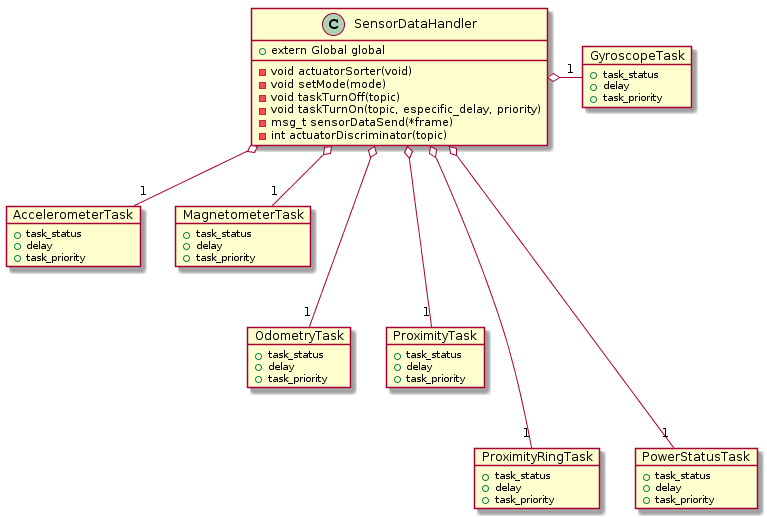
\includegraphics[width=15cm]{sensorclass}% 20cm, height = 10cm, angle = 90]{sensorclass}
  	\caption{SensorDataHandler.cpp and the sensor tasks structure}
  	\label{fig:sensorclass}
\end{figure}

\section{Overall functionality}
The sensor handler is a class which has only once instance and its started in the main class, along with the tasks for all the sensors inside each board. When the task for the sensor handler is started, it polls the CAN reception for a CAN frame that has the C\_S bit set to a '0' which corresponds to a \textit{Command data}, according to fig \ref{fig:can} of section \ref{sec:canconv}.

Whenever the sensor handler detects a CAN frame corresponding to a \textit{Command data}, the CAN frame has to be further analyzed to know if it is trying to communicate with a \textit{sensor} or with an \textit{actuator}. An example of this functionality can be seen in figure \ref{fig:seqoverall} which will be explained in section \ref{sub:rtimp}.

\subsection{Sensor data handling}
Whenever the command corresponds to a sensor, the next step is to read the DLC 0 to know if it is a command for stopping a sensor data, if it is a command for starting a publishing sensor data, or if it is a request for a one time transmission, see figure \ref{fig:sensormodes} from section \ref{sub:sensors}.

The state machine of figure \ref{fig:states} shows how the modes get handled. Whenever the DLC 0 has a '0' corresponding to a \textit{No transmission} is detected, the id from the topic gets identified and the corresponding task gets suspended so it no longer transmits its value.

When the DLC 0 has a '1' corresponding to a \textit{Publisher} is detected, the DLC 1, DLC 2, and DLC 3 get decoded to know the requested frequency from the id of the sensor that needs to start sending its information. If the sensor was already sending information, it needs to update its frequency and the priority, and it gets going.

Finally, when the DLC 0 has a '2' which means that the user wants a \textit{One time transmission} of a sensor data, this value gets sent one time only. If this sensor was sending its value in a publisher, then the task gets suspended.

\begin{figure}[ht]
 \centering
 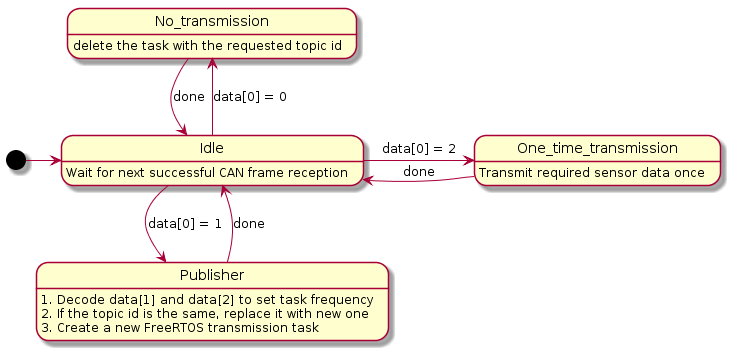
\includegraphics[width=\textwidth]{states}
		\caption{Modes implementation}
		\label{fig:states}
\end{figure}

\subsection{Actuator data handling}
In the other case, when the command is trying to communicate with an actuator, it goes into a sorter that separates the motor's command from the LEDs' command. If it is a command for the motors, then the motors get set with the velocity requested in the CAN frame. When its a LEDs command, the selected LED gets turn on or changes its color with the \textit{RGB} code reviewed in section \ref{sub:CANleds}.

\subsection{Real-time implementation}
\label{sub:rtimp}
The tasks corresponding to the sensors can all be operating at once. The priority of the tasks is being handled as preemptive tasks. This means that if two tasks are racing for the processing time, the one with higher priority will be preempted. Also, if one task is asked to output its value at the same frequency as a task that is already outputting its value, the one with higher priority will be on schedule and the one with less priority can be delayed some $\mu s$.

Everything up to this point works as an independent sensor data handler. This means that the internal controller is encapsulated and complete. The only thing that can interact with the functioning system are commands in the CAN bus. For this purpose the MuRox board has to be set and running the Linux based Operating System. See next chapter for more information about how to debug and the functionality of the \textit{Reflective Operator} in general.

An example of how the controller and the \textit{Reflective Operator} are communicating can be seen in figure \ref{fig:seqoverall}. The three boards are constantly checking the CAN bus for a CAN id corresponding to a \textit{command}. Whenever the \textit{Reflective Operator} sends a command asking for the gyroscope value with a specific frequency, this CAN frame gets fetched by the \textit{DiWheelDrive} board and starts the thread of the gyroscope with the requested frequency and priority.

In the image the \textit{Reflective Operator} asks then for a proximity ring value. This sensor is located on the \textit{Power Management} board so this thread gets started by this board. Afterwards, the \textit{Reflective Operator} asks to set the motor with a specific speed. The \textit{DiWheelDrive} board where the motors are connected, fetches this information and sets the motors accordingly.

The same process gets carried out for the odometry value request, which is managed also by the \textit{DiWheelDrive} board. The \textit{Reflective Operator} asks to stop the gyroscope sensor from sending its value. This command also gets fetched by the same board and puts the corresponding thread to sleep.

Finally the \textit{Reflective Operator} asks for the LED number 3 to turn on with a specific RGB value. This information is fetched by the \textit{Light Ring} board and turns on the LED with the requested information.

\begin{figure}[ht]
 \centering
 \caption{Functionality of an example application}
 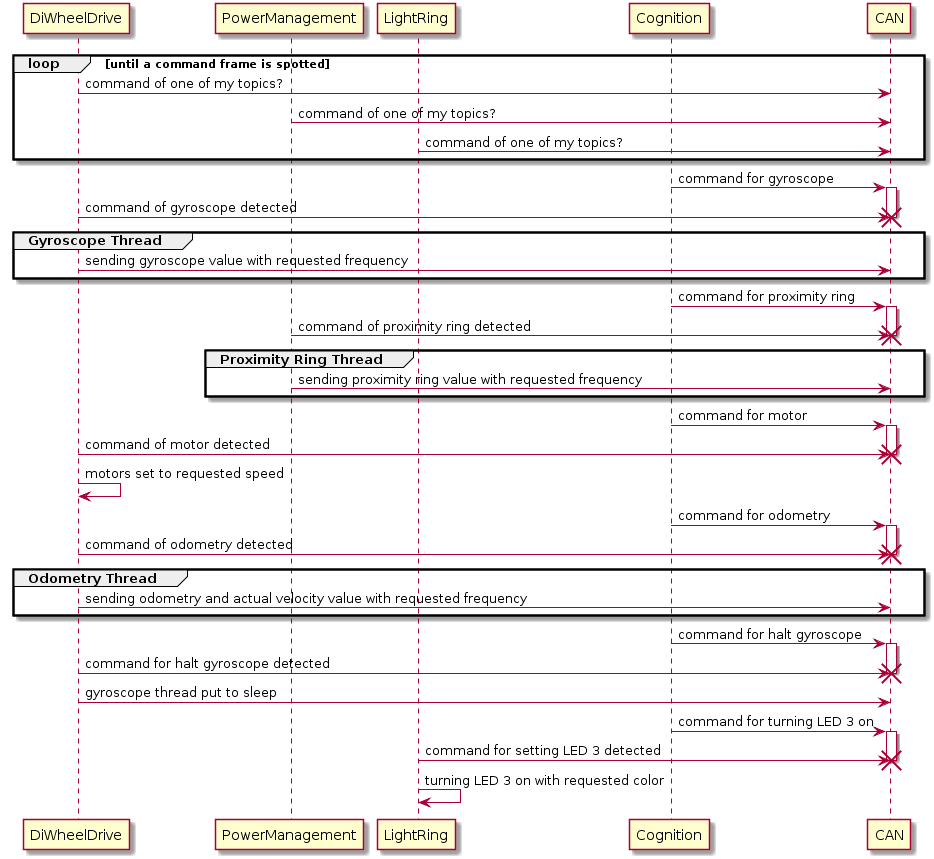
\includegraphics[width=\textwidth, height=18cm]{sequence_overall}
		\label{fig:seqoverall}
\end{figure}

\chapter{Reflective Operator}
\label{chap:reflective}
The board responsible of performing as the \textit{Reflective Operator} of the system is the MuRoX board. This board is the one that asks for a certain sensor data from the internal controller or also it can control the actuators. The user can connect to this board through ssh, with the address 192.168.1.1 with password \textit{root}.

The board already has a package called 'candump' which interacts with the CAN module in the board and can be used to debug the internal controller's functionality. The way of sending CAN frames from the MuRoX board has to follow the next convention:

\begin{lstlisting}[caption = CAN send format, label = CAN:debug, captionpos = b]
cansend can0 --identifier=CANid DLC0 DLC1 DLC2 DLC3 DLC4 ...
\end{lstlisting}

\section{Compiling for MuRoX}
\label{sec:poky}
For creating an application that the \textit{Reflective Operator} can run, it is necessary to use the \textit{cortexa8hf-vfp-neon-poky-linux-gnueabi} version of the cross-compiler. Once the application is compiled, the resulting binaries can be moved into the board using the \textit{scp} command.

\begin{lstlisting}[caption = moving files into MuRoX board \cite{AMiRo_Murox}, label = CAN:debug, captionpos = b]
scp anyFile root@192.168.0.1:~
\end{lstlisting}

\section{Compiling from a Simulink model for MuRoX}
\label{sec:matlab}
Alternatively, an application for the \textit{Reflective Operator} can be also compiled form a Simulink model. For this purpose, the user can modify the Simulink model that is already a part of the project, inside the \textit{Reflective\_Operator/Matlab\_Reflective\_Operator} from figure \ref{fig:DAAMIROstr}. Once the model has been edited, the user has to generate the code using the Matlab solver with the current settings.

After the code has been successfully generated, the user must go into the \textit{Reflective\_Operator/Demo\_Applications/Demo\_Matlab\_Reflective\_Operator} directory where a bash file with the name of \textit{matlab\_amiro\_setup.sh} is. When executed, this shell script copies the necessary files into the current folder, copies a custom makefile that was created to cross-compile with the requirements for the MuRoX board, and compiles the application. The generated binary can be copied into the MuRoX board with the method described in section \ref{sec:poky}.

\section{Example applications}
\label{sect:example}
For testing purposes, four demo applications were created. These applications are already inside the \textit{Reflective Operator}, but the user can modify and recompile the source code which is obtainable from the DA\_AMiRo git repository \cite{AMiRo_Git}. The modified versions of the source code can be compiled and uploaded to the MuRoX board using the method already described in section \ref{sec:poky}. The three demos are:

\begin{itemize}
  \item \textit{Demo Sender Reflective Operator}
  \item \textit{Demo Receiver Reflective Operator}
	\item \textit{Demo Standalone Reflective Operator}
	\item \textit{Demo Matlab Reflective Operator}
\end{itemize}

The first one is called \textit{Demo Sender Reflective Operator} and it is a simple application where the user can send commands to the internal controller with assistance of a set of menus. The application asks for the priority, the topic id, the mode to be set, and all the needed fields for each case. It also separates actuators from sensors. This application facilitates the sending of commands, because the user does not have to memorize the topic ids or the CAN frame conventions.

In figures \ref{fig:sender1} and \ref{fig:sender2} a possible usage of the demo is shown. The menus can be seen, as the first one asks if the user wants to talk with an actuator or a sensor. If the answer is an actuator, like in figure \ref{fig:sender1} the second menu is to select which actuator to use and finally to set the according values to the desired actuator. If the user wants to talk with a sensor like in figure \ref{fig:sender2}, the menus ask for the mode: stop, publisher, and one time transmission. Then it proceeds to ask the frequency if it was publisher, the topic and the priority.

\begin{figure}[ht]
 \centering
 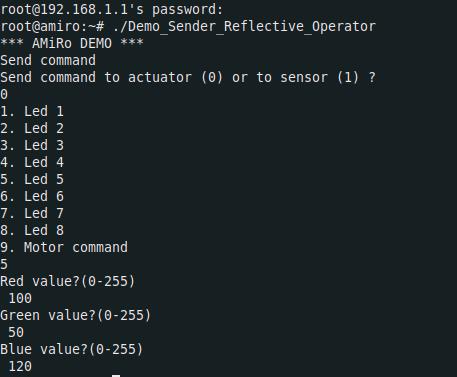
\includegraphics[width=\textwidth, height=8cm]{sender_example2}
		\caption{Example of a \textit{Demo Sender Reflective Operator} usage, part 1}
		\label{fig:sender1}
\end{figure}

\begin{figure}[h]
 \centering
 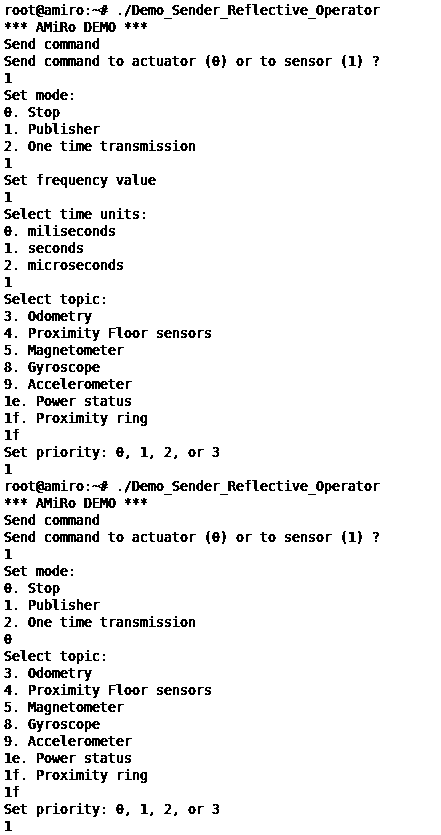
\includegraphics[width=\textwidth, height=18cm]{sender_example}
		\caption{Example of a \textit{Demo Sender Reflective Operator} usage, part 2}
		\label{fig:sender2}
\end{figure}

The second application is called \textit{Demo Receiver Reflective Operator} and it is basically a thread that outputs the information that the CAN bus receives corresponding to the sensors. The information is translated in English so the user can read it easily without the necessity of the convention shown in figures \ref{fig:can} and \ref{fig:sensormodes}. The output shows the priority, a time stamp upon the reception of the CAN frame, the topic of the sensor's data, the value, and its units. This can be seen in figure \ref{fig:receiver1}, where an example of how the receiver displays the information of the gyroscope can be seen.

\begin{figure}[ht]
 \centering
 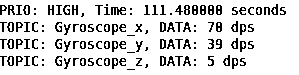
\includegraphics[]{receiver_example}
		\caption{Example of a \textit{Demo Receiver Reflective Operator} for the gyroscope}
		\label{fig:receiver1}
\end{figure}

The idea behind these two applications \textit{Demo Sender Reflective Operator} and \textit{Demo Receiver Reflective Operator} is that the user runs both at the same time in two different terminal windows to send commands and to see how they are being answered in real time.

The third application is called \textit{Demo Standalone Reflective Operator}. It has a determined functionality so the user needs only to run it in order to see its results with the help of the \textit{Demo Receiver Reflective Operator} or the \textit{candump} package. This Demo has a set of commands to be sent to the internal controller and shows the outputs of the sensors. The demo has the following expected functionality which can be seen in figures \ref{fig:timing1} and \ref{fig:timing2}.

\begin{enumerate}
\item At 1s the CAN bus has a command frame asking for the accelerometer values every 500ms.
\item At 5s the CAN bus has a command frame asking for the proximity ring values every second.
\item At 10s the CAN bus has a command frame asking for the power status one time.
\item At 15s the CAN bus has a command frame asking for the gyroscope values every 5s.
\item At 16s the CAN bus has a command frame asking for the proximity ring values to stop being transmitted.
\item At 17s the CAN bus has a command frame asking for the magnetometer values every 800ms.
\item At 18s the CAN bus has a command frame asking for the accelerometer values to stop being transmitted.
\item At 21s the CAN bus has a command frame asking for the odometry values every 900ms.
\item At 23s the CAN bus has a command frame asking to set the motors speed at 50$\mu m/s$.
\item At 25s the CAN bus has a command frame asking to turn LED 1 on.
\item At 27s the CAN bus has a command frame asking to stop the motors.
\item At 30s the CAN bus has a command frame asking for the odometry values to stop being transmitted.
\item At 31s the CAN bus has a command frame asking for the power status one time.
\item At 33s the CAN bus has a command frame asking for the proximity floor values every 2s.
\item At 35s the CAN bus has a command frame asking for the magnetometer values to stop being transmitted.
\item At 38s the CAN bus has a command frame asking for the proximity ring values to stop being transmitted.
\item At 40s the CAN bus has a command frame asking to turn LEDs 2, 4, 6, and 8 on.
\end{enumerate}

\begin{figure}[ht]
	\centering
	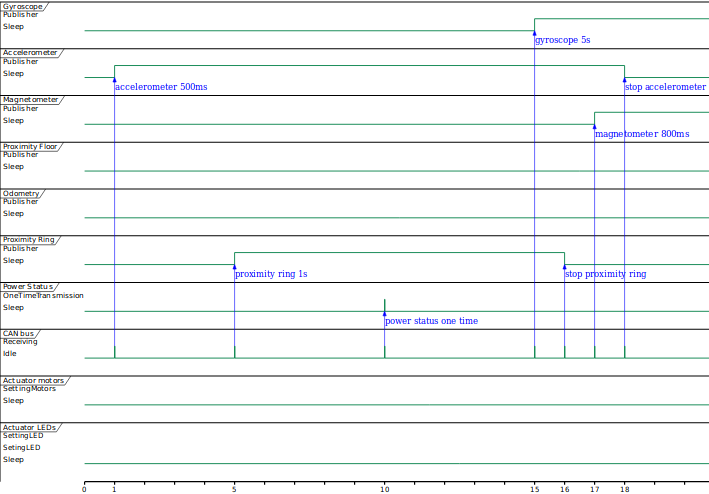
\includegraphics[width=\textwidth, height=13cm]{timing_1}
  	\caption{Demo Standalone sequence part 1}
  	\label{fig:timing1}
\end{figure}

\begin{figure}[h]
	\centering
	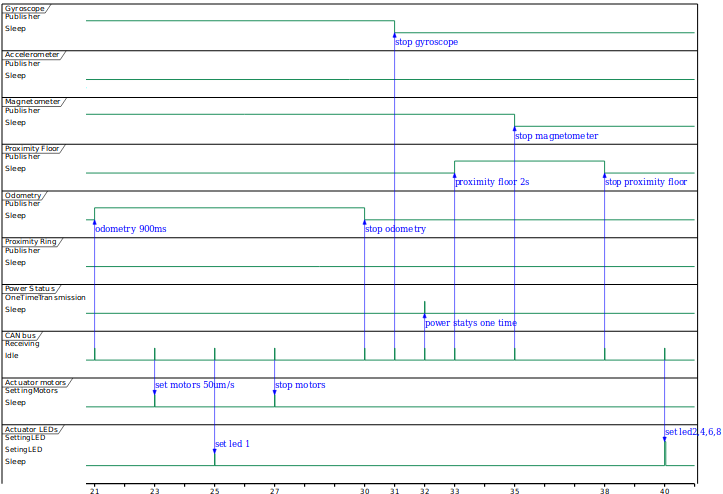
\includegraphics[width=\textwidth, height=13cm]{timing_2}
  	\caption{Demo Standalone sequence part 2}
  	\label{fig:timing2}
\end{figure}

The fourth demo is the \textit{Demo Matlab Reflective Operator} and it is the resulting application from the Simulink model. The current demo turns on three LEDs on the AMiRo but the user can modify the Simulink model to fulfill any desired functionality. The way of compiling a modified version of the Simulink model was discussed in section \ref{sec:matlab}.

Lastly, the user can also send independent CAN frames using the \textit{candump} package installed in the MuRoX board, as it was already discussed in chapter \ref{chap:reflective}. For this method, the user has to decode previously the topic id and the CAN data frames according to images \ref{fig:can} and \ref{fig:sensormodes}.

\chapter{Results}
\section{DA\_AMiRo performance}
In this section the performance of the AMiRo will be revised based the results of some testing conducted to the AMiRo. From all the testing conducted, the AMiRo's response to the \textit{Demo Standalone Reflective Operator} will be the one discussed in this section, because its desired functionality was already explained in section \ref{sect:example}.

\begin{figure}[ht]
	\centering
	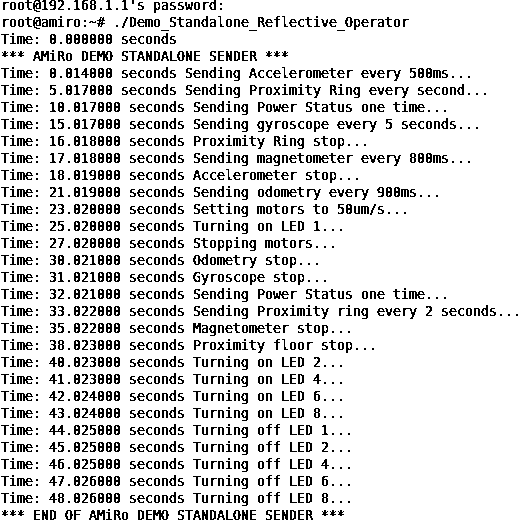
\includegraphics[width=\textwidth, height=15cm]{standalone_sender}
  	\caption{Demo Standalone results sender part}
  	\label{fig:ressend}
\end{figure}

\begin{figure}[ht]
	\centering
	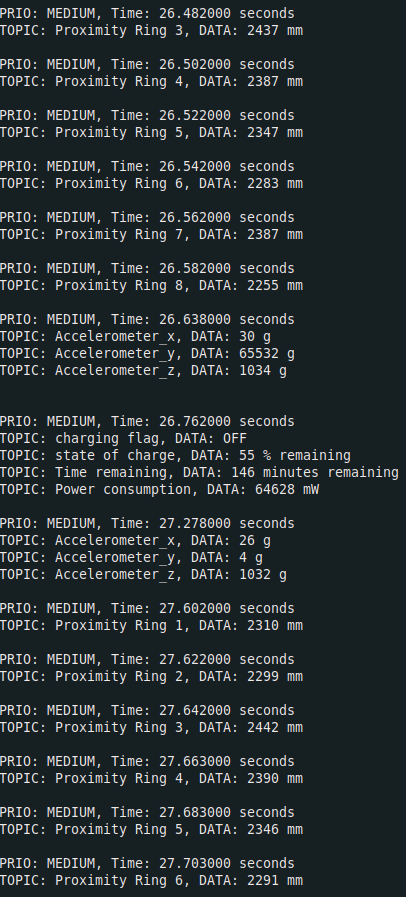
\includegraphics[width=\textwidth, height=15cm]{standalone_1}
  	\caption{Demo Standalone results part 1}
  	\label{fig:res1}
\end{figure}

\begin{figure}[ht]
	\centering
	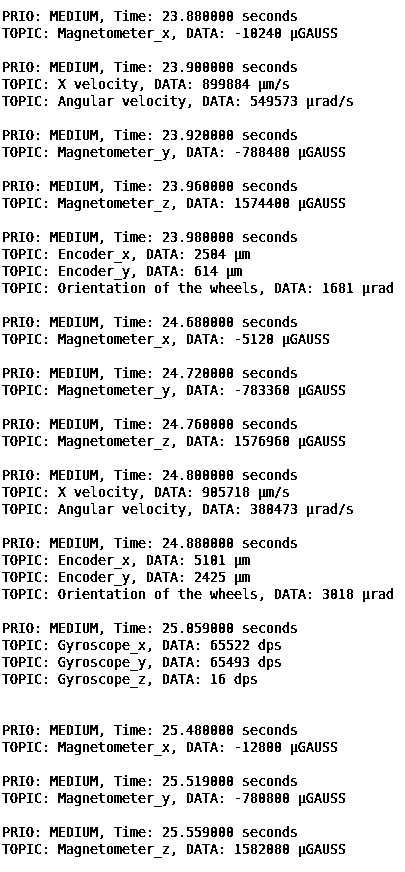
\includegraphics[width=\textwidth, height=18cm]{standalone_2}
  	\caption{Demo Standalone results part 2}
  	\label{fig:res2}
\end{figure}

\begin{figure}[ht]
	\centering
	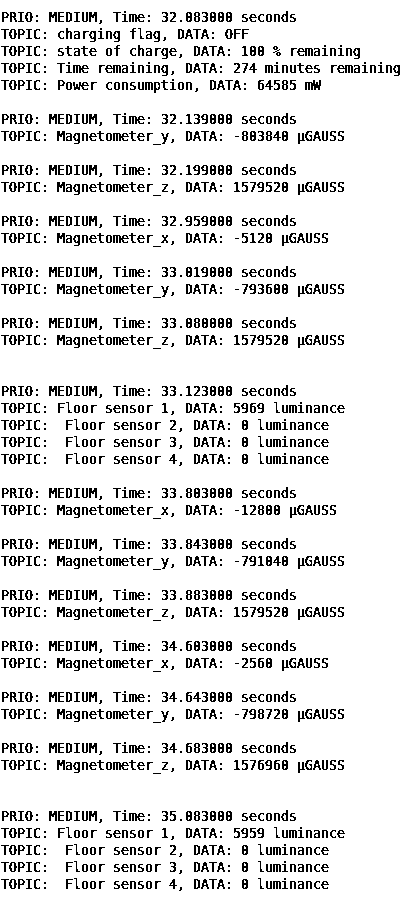
\includegraphics[width=\textwidth, height=18cm]{standalone_3}
  	\caption{Demo Standalone results part 3}
  	\label{fig:res3}
\end{figure}

In figure \ref{fig:ressend} the process described in figures \ref{fig:timing1} and \ref{fig:timing2} is shown and it displays the expected behavior of the \textit{Demo Standalone Reflective Operator}. This figure also have time stamps corresponding to the time at which each CAN frame was sent to the CAN bus. Among the listing of commands that are sent to the CAN bus by this application, the reader can also look at the actuators commands such as the motor's velocity and the turning on and off of the LEDs.

Now lets have a look at the results. In figure \ref{fig:res1} the values of the accelerometer and the proximity ring sensors are displayed. In figure \ref{fig:res2} values for the magnetometer, gyroscope, velocity, and encoders are displayed. The velocity and encoder CAN frames show that the motors were on-going at the moment of the CAN frame being sent. And finally in figure \ref{fig:res3} the power status gets shown, the magnetometer values appear as well, and also the proximity floor sensors are displayed.

The functionality and frequency of the expected values is very satisfactory, because the delays between every value from the same sensor are exactly as the requested in the \textit{Demo Standalone Reflective Operator} seen in figure \ref{fig:ressend}. And even though as seen on top of figure \ref{fig:res2}, the CAN frames for the magnetometer values are not sent in a row but the value of the velocity gets sent before the magnetometer 'y' value. This behavior is expected as it adheres to the requested frequencies. In the case from the velocities requested frequency, the $900ms$ between two velocity CAN frames is precise.

As it can be seen, the delay between two CAN frames of the same sensor, correspond to the frequencies requested from the \textit{Demo Standalone Reflective Operator} as seen in figure \ref{fig:ressend}. There is however, an expected delay between the sensors that get sent together in different CAN frames. Such is the case of the magnetometer values, that are sent in three different CAN frames and the proximity floor ring sensors that are sent in eight different CAN frames as explained in section \ref{sub:sensors}. This delay is of $20ms$ and affects only the frequencies of said  sensor values. So for example if the magnetometer value gets requested at a period of time shorter than every $20ms$, then the CAN frames will not be sent appropriately. This delay does not affect other possible parallel tasks.

For starters, lets look into the DA\_AMiRo efficiency. From the programming of the three basic boards, a $545\mu s$ delay of timeouts in every transmission is expected. This number can be explained with the following equation: $$1 us   (1+11+1+1+1+4+64+15+1+1+1+7)*5= 545 us$$ $$1/(1MHz)*(SOF+ID+RTR+IDE+RES+DLC+DATA+CRC+$$ $$DELIM+ACK+DELIM+EOF)*No. RETRIES$$
taken from the original code of the repository \cite{AMiRo_Wiki}.

\section{DA\_AMiRo vs. AMiRo OS}
In this section the structure and functionality of the AMiRo OS and the OCM approach for the DA\_AMiRo project are compared.

The AMiRo OS is a very complete system that has a lot of possible applications for different purposes, from line followers, to a LIDAR that can detect obstacles. It also has a command line shell in which the user can communicate with the AMiRo in very simple commands. This feature is very helpful to get an immediate status of a sensor or to get a quick response from the AMiRo.

Every board has a user thread where a functionality using the sensors of the board is implemented. Everyone of these boards gets to broadcast its sensor values via CAN with a pre-selected frequency. A good way the user can interact with the sensors and the boards themselves, is via the \textit{Cognition Board} that also has pre-compiled demos in the Wiki \cite{AMiRo_Murox} for different possible applications.

The AMiRo OS has all of the possible functionalities already implemented and this takes a lot of the processing power from the boards, this is one of the main differences between this and the DA\_AMiRo project. The latter has a specific purpose and the processing power is focused towards this goal, making it more resource effective. A good example of this is that the DA\_AMiRo does not have possible demos implemented like the line follower, the motor corrections, and the obstacle avoidance for mentioning a few.

What appears to be similar between these two projects is the CAN broadcasting of the AMiRo OS and the CAN sensor handler of the DA\_AMiRo project. The AMiRo OS sends the values of the sensors all together via the CAN bus at a specific frequency of $16Hz$, while the DA\_AMiRo project has a much more complex sensor value handling as it has been already explained through the past chapters.

One of the biggest advantages of the DA\_AMiRo project is the compatibility of the Simulink models from Matlab to generate applications for the Reflective Operator of the AMiRo. The students can easily edit the given model to operate according a desired goal. This method is easy because with the Simulink model the students can change logic in a visual fashion rather than a code one. Instead of having to remember the CAN frame conventions or worrying about a programming language issue, they can simply change the values of the model or create logic with simple block logic in Simulink.

\section{Outlook}
The real-time functionality in the DA\_AMiRo project is works as expected: it fulfills the performance deadlines and does not loose packages. After performing a stress test on the system, the error range or delays found are still small enough to make the project fulfill the requirements of a soft real-time system.

The system is also capable of handling all the available tasks from the sensors at once, and communicates successfully with the actuators, changing its values at the will of the user. On top of this, the DA\_AMiRo project is fulfilling the CAN frame conventions established by Uwe Jahn.

With the help of the Simulink models, the usage of the Reflective Operator becomes very simple. This feature makes the DA\_AMiRo project a good tool for students to work with real-time systems and learn from them in a simple and visual way.

%bibliography
\printbibliography
\nocite{*}

\end{document}
\grid
